\chapter{Ergebnisse}
In diesem Kapitel werden die Ergebnisse numerischer Experimente für das Schema aus Abschnitt \ref{sec:primal} vorgestellt. Tabelle \ref{tab:parameter} listet die einstellbaren Parameter mit einer kurzen Beschreibung und ihren Default-Werten auf.
\begin{table}
  \centering
  \caption{Einstellbare Parameter und ihre Default-Werte.}
  \label{tab:parameter}
  \sisetup{parse-numbers=false}
  \scriptsize
  \begin{tabular}{p{0.1\textwidth} p{0.65\textwidth} p{0.1\textwidth}  }
    \toprule
    {Symbol} & Beschreibung & Default \\
    \midrule
       & \emph{Physikalische Parameter} & \\
    $L_x$ &Länge des Rechengebietes in $x$-Richtung & $\SI{106}{\nano\meter}$ \\
    $L_y$ &Länge des Rechengebietes in $y$-Richtung & $\SI{130}{\nano\meter}$ \\
    $L_D$ & Ausdehnung des Spannungsabfalls (s. Abbildung \ref{fig:pot1}) & $\SI{26}{\nano\meter}$\\
    $L_1$ & Abstand der Potentialbarrieren (s. Abbildung \ref{fig:pot1}) &$\SI{6}{\nano\meter}$ \\
    $L_2$ & Breite der Potentialbarrieren  (s. Abbildung \ref{fig:pot1}) &$\SI{4}{\nano\meter}$ \\
    $V_0$ & Barrierenhöhe (Differenz der Leitungsbandkantenenergien) &$\SI{0.2098}{\electronvolt}$ \\
    $N_D$ & Donatorkonzentration des GaAs & $10^{24}\,\text{m}^{-3}$ \\
    $m$ & Effektive Elektronenmasse in GaAs & $0,063 m_e$ \\
    $\mu$   & Chemisches Potential (wird errechnet, siehe Abschnitt \ref{sec:A_3}) & $\SI{46}{\milli\electronvolt}$ \\
    $\delta$ & Einflussbereich des ac{cap}, siehe Gleichung \eqref{eq:cap} & $0,2 L_y$\\
    $W_0$ & Stärke des \ac{cap}, siehe Gleichung \eqref{eq:cap} &$-1V_0$ \\
    $U$   &Spannung, die über die Strecke $L_D$ abfällt & $\SI{0}{\volt}$ \\
    \midrule
     & \emph{Parameter der Numerik} & \\
    $K_x$ & \# Zellen der \ac{dg}-Diskretisierung & 60 \\
    $K_y$ & \# Zellen der \ac{fv}-Diskretisierung & 100 \\
    $N$ & Polynomgrad der \ac{dg}-Diskretisierung & 2 \\
    $N_q$ & Quadraturordnung für Methode G2 & 20 \\
    $\kappa$ & Strafparameter des numerischen Flusses, siehe Gleichung \eqref{eq:numflux} &$\nicefrac{1}{2}$ \\
    \midrule
     & \emph{Parameter des Programmablaufs} & \\
    doGL & Soll Methode G2 verwendet werden?(sonst G1) Die Quadraturordnung ist stests 20. & true \\
    doPotConv & Soll das Potential mit einer Gaußverteilung gefaltet werden? & false\\
    withCAP & Soll das \ac{cap} eingeschaltet werden? & true \\
    doTransient & Soll transient gerechnet werden? & false \\
    doGummel & Soll selbstkonsistent gemäß den Erläuterungen in Kapitel \ref{sec:A_4} gerechnet werden? & false \\
    Nrefine  & \# Verfeinerungen in der Polynomordnung $N$ mit $N_{i+1}=N_i+1$ & 0 \\
    Krefine  & \# Verfeinerungen in der Anzahl Elemente $K_x$ mit $K_{x,i+1}=2K_{x,i}$ & 0 \\
    \bottomrule
  \end{tabular}
\end{table}
Offenbar entsteht eine große Variationsmöglichkeit. Zunächst soll jedoch im nächsten Abschnitt die Funktionalität des Schemas getestet werden für ein analytisch lösbares Randwertproblem. Daraufhin wird die stationäre Lösung näher untersucht. Der mit der Elektronendichte korrespondierende Realteil sowie der mit dem Strom korrespondierende Imaginärteil werden für verschiedene Spannungen gezeigt. Aus einer Mittelung des Stromes über $x$ ergibt sich der Gesamtstrom in Abhängigkeit von der Spannung. Hierfür soll in Kapitel \ref{sec:IV} insbesondere der Einfluss der physikalischen Längen sowie die Übereinstimmung mit der Erwartung gemäß Abbildung \ref{fig:IVkurve} untersucht werden. Besonders interessant sind darüber hinaus Fehlerraten, die eine Aussage über die Qualität des verwendeten Verfahrens liefern. Dazu wird in Kapitel \ref{sec:rates} einerseits ein Vergleich mit der \ac{tf} aus Kapitel \ref{sec:TFmethod} gezogen, andererseits eine iterative Fehlerrate definiert. Abgeschlossen wird das Kapitel durch eine Untersuchung der transienten Lösung in Abschnitt \ref{sec:transient}.

\section{Notation}\label{sec:notation_4}
Für numerische Untersuchungen ist die Definition eines \emph{analytischen Fehlers} \index{analytischer Fehler}
\begin{equation}
  e_{\nicefrac{i}{r}}^{\alpha} = \norm{\nicefrac{\operatorname{Re}}{\operatorname{Im}} (u - u\fin^{\alpha})}_{L^2(\Omega)}
  \label{eq:error_ana}
\end{equation}
sowie eines \emph{iterativen Fehlers}\index{iterativer Fehler}
\begin{equation*}
  e_{\mathcal{T}, \nicefrac{i}{r}}^{\alpha} = \norm{\nicefrac{\operatorname{Re}}{\operatorname{Im}} (u\fin^{\alpha} - u\fin^{\alpha-1})}_{L^2(\Omega)}
\end{equation*}
sinnvoll, wobei $\Omega=\Omega_x \times \Omega_y$ das Rechengebiet, $u$ die exakte Lösung und $u\fin$ die Ritz-Approximation sind. Der Index $\alpha>0$ bezieht sich auf die Verfeinerung des Gitters in $x$-Richtung gemäß $K_x^{\alpha} = 2^\alpha$. Wenn nicht anders angegeben, werden die benötigten Integrale in $x$-Richtung mit Gauß-Lobatto Quadratur der Ordnung $N$ (also gleich der Ordnung des \ac{dg}-Verfahrens) berechnet.
In $y$-Richtung hingegen wird schlicht $\int_{\Omega_y}\diff y f(y) \approx \sum_{j=1}^{K_y} h_y f(y_j)$ berechnet, da $f(y)$ im \ac{fv}-Verfahren konstant ist innerhalb der Zelle $j$.

Für die Betrachtung der \emph{Konvergenzordnung}\index{Konvergenzordnung} in Abschnitt \ref{sec:rates} werden ferner die Fehlerraten
\begin{equation}
  \begin{aligned}
    r_{\nicefrac{i}{r}}^{\alpha} &= \frac{\ln(e_{\nicefrac{i}{r}}^{\alpha}) - \ln(e_{\nicefrac{i}{r}}^{\alpha-1})}{\ln(K_x^{\alpha-1}) - \ln(K_x^{\alpha})} \qquad\text{und}\\
    r_{\mathcal{T},\nicefrac{i}{r}}^{\alpha} &= \frac{\ln(e_{\mathcal{T},\nicefrac{i}{r}}^{\alpha}) - \ln(e_{\mathcal{T},\nicefrac{i}{r}}^{\alpha-1})}{\ln(K_x^{\alpha-1}) - \ln(K_x^{\alpha})}
  \end{aligned}
  \label{eq:fehlerraten}
\end{equation}
definiert. Daraus lassen sich noch $r_{\nicefrac{i}{r}}$ bzw. $r_{\mathcal{T},\nicefrac{i}{r}}$ als Mittelwerte über $\alpha$ errechnen. Die Definition der Fehlerrate ist motiviert durch eine Fehlerabschätzung der Form $e \leq ch_x^r$. Logarithmieren und Subtrahieren für zwei verschiedene mittlere Gitterabstände $h_x$ liefert die Konvergenzordnung $r$.

Wann immer die numerische Lösung $u\fin$ ausgwertet werden muss, sind die Gleichungen\eqref{eq:ellPsi} und \eqref{eq:vandermonde} hilfreich. Sei nun $u\fin$ an der Stelle $x_0$ auszuwerten. Dann ist zunächst das Element $D^k$ zu suchen, für das $x_0\in D^k$ gilt. Durch Gleichung \eqref{eq:affmap} ergibt sich hieraus $r_0$ als Koordinate auf dem Referenzelement $I$. Dann gilt nach Gleichung \eqref{eq:nodal}
\begin{align*}
  v\fin(x_0) &= v\fin^k(r_0,t) = \sum_{j=1}^{N_p} v_{\mathcal{T},j}^k(t)\ell_j(r_0) \\
   &\stackrel{\eqref{eq:ellPsi}}{=} \sum_{j=1}^{N_p} v_{\mathcal{T},j}^k(t) ((\van^T)^{-1}\Psi(r_0))_j \; .
\end{align*}
Jetzt wird eine weitere Vandermondematrix $\tilde{\van}$ der Dimension $1\times N_p$ eingeführt, um den Punkt $r_0$ zu errechnen. Nach Gleichung \eqref{eq:vandermonde} ist also $\tilde{\van}_{1j}=\Psi_j(r_0)$. Dann folgt
\begin{align*}
  v\fin(x_0) &= \sum_{i=j}^{N_p} v_{\mathcal{T},j}^k(t) ((\van^T)^{-1}\tilde{\van}^T)_{j,1} \\
  &= (\tilde{\van}\van^{-1})\underline{v}_j^k(t) \; ,
\end{align*}
wobei im letzten Schritt die Definition \ref{def:matrizen} sowie die Vertauschbarkeit von Invertierung und Transponierung einer Matrix eingegangen sind. Falls $r_0\in\{-1,1\}$, so ist $u\fin$ auf einer Kante auszuwerten. An diesen Stellen wird der numerische Fluss verwendet. Anhand des Vorzeichens des zu $y_j$ korrespondierenden Eigenwerts $\lambda_j$ aus Gleichung \eqref{eq:Lambda} wird entweder $u\fin^+$ oder $u\fin^-$ ausgewertet, siehe auch Abbildung \ref{fig:notation_DG}.

Die soeben angestellten Überlegungen zur Auswertung der numerischen Lösung mögen aufwändig erscheinen. Wenn jedoch Fehlerraten bestimmt werden sollen, ist die exakte Auswertung nach Ansicht des Autors unerlässlich. Eine interpolatorische Bestimmung der $L^2$-Norm führt ansonsten zu Abweichungen. Insbesondere für grobe Diskretisierungen (also kleine Werte von $K_x$, $N$) sind diese deutlich zu spüren.

\section{Test für ein analytisch lösbares Randwertproblem}\label{sec:test}
Losgelöst von der physikalischen \ac{lvn} wird in diesem Abschnitt für Testzwecke die Gleichung \eqref{eq:qschema} mit
\begin{equation*}
  \begin{aligned}
    A^y& = 0 \\
    B^y_{j,j} &= -1/a(y_j) \qquad \text{mit} \;\; a(y)=\sin\left(\frac{2\pi y}{L_y}\right) \\
    C^y_{j,j} &= i
  \end{aligned}
\end{equation*}
mit äquidistanten $y_1,\dots,y_{K_y}=-L_y/2,\dots,L_y/2$ betrachtet. Unter den Randbedingungen
\begin{equation*}
  \begin{aligned}
    u(x,y)|_{\partial \Omega} = \exp(ia(y)x)
  \end{aligned}
\end{equation*}
entspricht die analytische Lösung der Gleichung \eqref{eq:qschema} eben dieser Funktion, also $u(x,y) = \exp(ia(y)x)$ auf ganz $\Omega$. Für die diagonalisierte Gleichung \eqref{eq:diagLVN} ist mit $v_t=0$ die Geschwindigkeit $\Lambda^y=B^y$ und der Driftoperator $G=C^y$. Die Systemmatrix aus Abschnitt \ref{sec:implementierung} wird entsprechend angepasst.

Nun liegt der sehr einfache Fall von $K_y$ entkoppelten Advektions-Reaktions Gleichungen vor. Aus der umfangreichen Literatur kann beispielsweise in \cite{lesaint1974finite} die \emph{a priori} Fehlerabschätzung
\begin{equation}
  e \leq c h_x^{N_x + 1} \label{eq:optimaleKonvergenz}
\end{equation}
gefunden werden, falls $u \in H^{N_x+2}$ liegt, was für die obige Lösung in der Tat gilt. Diese Konvergenzordnung ist optimal und lediglich für reinen Upwind Fluss in linearen Problemen gültig. Die Abbildung \ref{fig:testResult} zeigt die im vorherigen Abschnitt definierten Fehler in Abhängigkeit von Polynomgrad und Anzahl der Elemente.
\begin{figure*}
    \centering
    \begin{subfigure}[b]{0.475\textwidth}
        \centering
        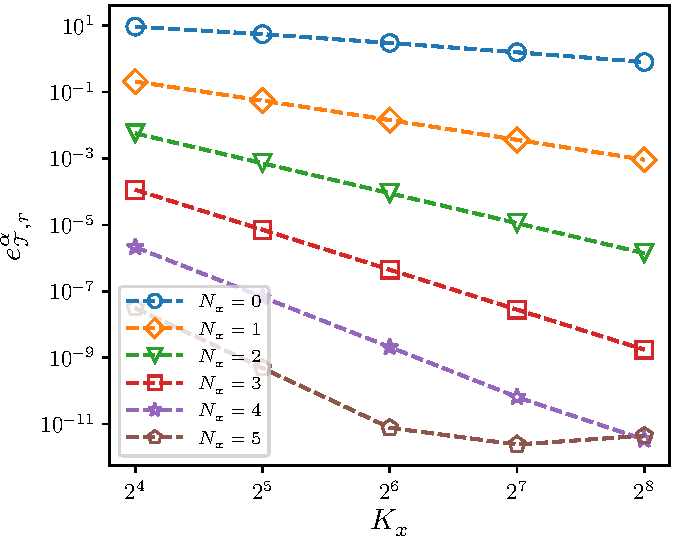
\includegraphics[width=\textwidth]{plots/test1_r.pdf}
        \caption[]%
        {{\small Analytischer Fehler $e_r$.}}
    \end{subfigure}
    \hfill
    \begin{subfigure}[b]{0.475\textwidth}
        \centering
        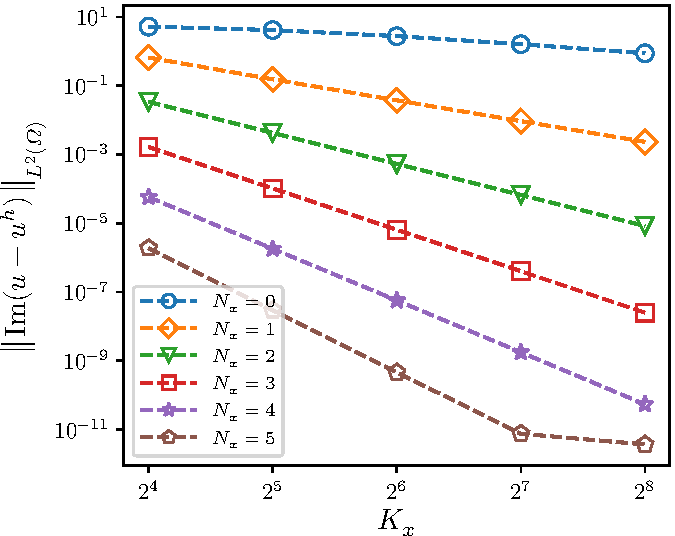
\includegraphics[width=\textwidth]{plots/test1_i_rel.pdf}
        \caption[]%
        {{\small Iterativer Fehler $e_{\mathcal{T},i}$.}}
    \end{subfigure}
    \caption[]
    {Fehler in Abhängigkeit von Polynomgrad $N$ und Anzahl Elemente $K_x=2^{\alpha}$ mit $K_y=50$. Die Steigung der Geraden stellt die Fehlerrate dar, welche hier optimal ist. Bei $e\approx10^{-11}$ ist offenbar die CPU-Genauigkeit erreicht.}
    \label{fig:testResult}
\end{figure*}
Es zeigt sich optimale Konvergenz nach Gleichung \eqref{eq:optimaleKonvergenz} mit
\begin{align*}
  r_r &= \{0.86\pm0.07,\; 1.94\pm0.03,\; 3.0\pm0.0,\; 4.0\pm0.0,\; 5.0\pm0.0,\; 4.55\pm2.04\} \\
  r_i &= \{0.83\pm0.08, 1.95\pm0.03, 3.0\pm0.0, 4.0\pm0.0, 5.0\pm0.0, 4.6\pm1.97\} \\
  r_{\mathcal{T},r} &= \{0.63\pm0.16, 2.06\pm0.05, 3.0\pm0.0, 4.0\pm0.0, 5.0\pm0.0, 5.97\pm0.04\} \\
  r_{\mathcal{T},i} &= \{0.57\pm0.18,\; 2.05\pm0.04,\; 3.0\pm0.0,\; 4.0\pm0.0,\; 5.0\pm0.0,\; 5.97\pm0.04\}
\end{align*}
jeweils für $N=\{0,\dots,5\}$. Imaginärteil und Realteil zeigen keine erkennbaren Unterschiede auf. Der Einbruch für feine Diskretisierungen ist der endlichen CPU-Genauigkeit zuzuschreiben.

\section{Observablen der stationären Lösung}\label{sec:IV}
Die in Kapitel \ref{sec:2_1} eingeführten Observablen der Teilchendichte $n(x,t)$ nach Gleichung \eqref{eq:expval_n} und der Stromdichte $j(x,t)$ nach Gleichung \eqref{eq:expval_j} lassen sich aus der Dichtematrix auf einfache Weise gewinnen. Für die Stromdichte wird noch eine Ableitung bezüglich $y$ benötigt. Hierfür wird der Differenzenquotient gemäß
\begin{equation}
  \partial_y u\fin(x,y,t)|_{y=0} \approx\frac{1}{h_y}(u\fin(x,y_{K_y/2+1},t)-u\fin(x,y_{K_y/2},t))
  \label{eq:ableitung_y}
\end{equation}
gebildet. Da $K_y$ stets gerade gewählt wird, liegt die Kante zwischen den Elementen $K_y/2+1$ und $K_y/2$ genau bei $y=0$.

\subsection{Dichtematrix}
Ein erster Test des Verfahrens überprüft die Symmetrieeigenschaften der numerischen Lösung. Mit Hilfe von Gleichung \eqref{eq:Liouvilleoperator} ist in Kapitel \ref{sec:dynamik} gezeigt worden, dass die exakte Lösung im stationären Fall $u(x,y) = -u^*(x,-y)$ erfüllt. Die Differenz $(u\fin(x,y)-u\fin^*(x,-y))/\norm{u\fin(x,y)}_{L^2(\Omega)}$ ist in Abbildung \ref{fig:parity} gezeigt.
\begin{figure}
  \centering
  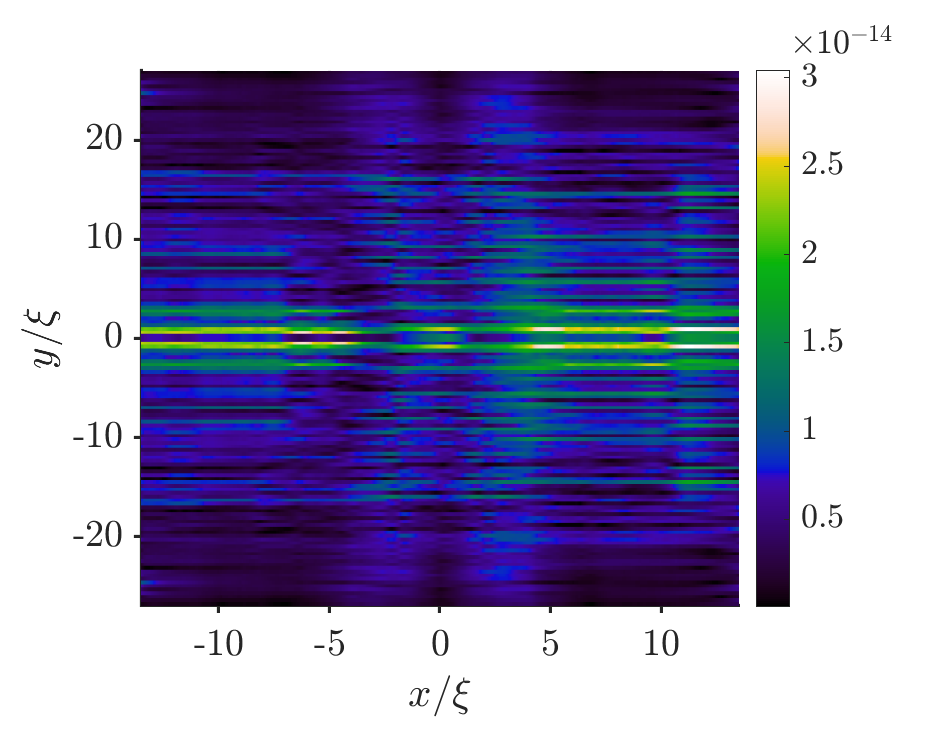
\includegraphics[width=0.5\textwidth]{plots/parity_abs.eps}
  \caption{Dargestellt ist die Differenz $|u\fin(x,y)-u\fin^*(x,-y)|/N_D$. Die Symmetrieanforderung  wird bis auf CPU-Genauigkeit erfüllt.}
  \label{fig:parity}
\end{figure}

Abbildung \ref{fig:solution} zeigt Real- und Imaginärteil der numerischen Lösung für zwei Spannungen $U_1=\SI{0}{\volt}$, $U_2=\SI{0.14}{\volt}$.
\begin{figure*}
    \centering
    \begin{subfigure}[b]{0.48\textwidth}
        \centering
        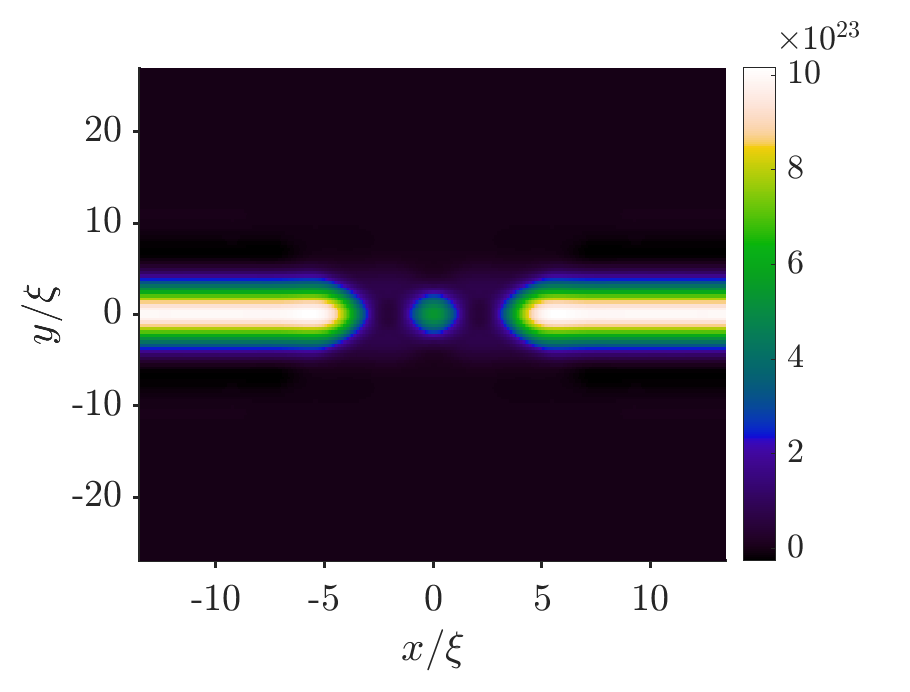
\includegraphics[width=\textwidth]{plots/section2/real_0.00V_Kx30_Nx4_Ky150_flat.eps}
        \caption[]%
        {{\small Realteil bei $U_1=\SI{0}{\volt}$.}}
        % \label{fig:G_1}
    \end{subfigure}
    \hfill
    \begin{subfigure}[b]{0.48\textwidth}
        \centering
        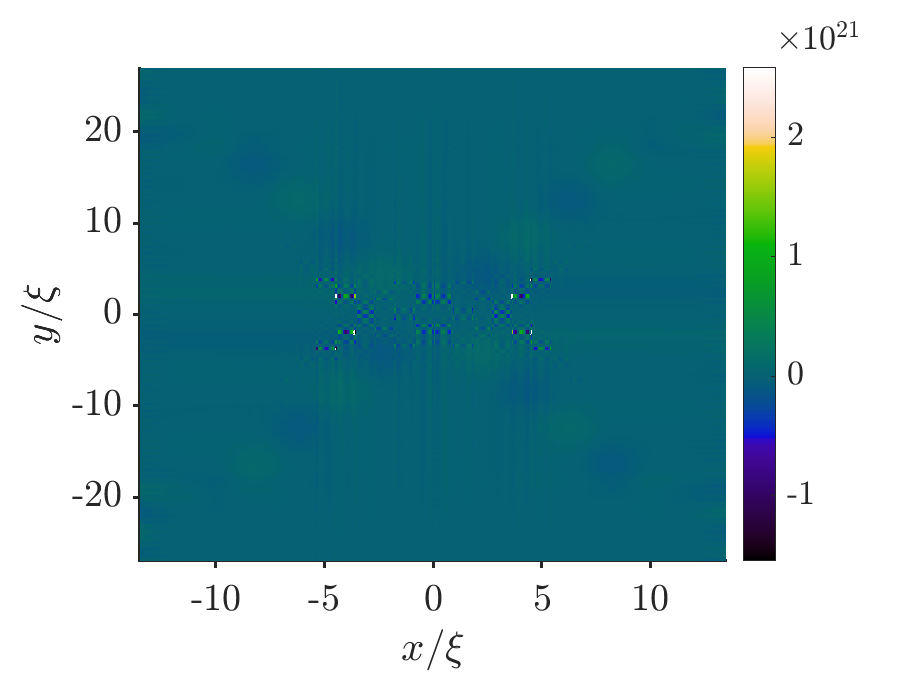
\includegraphics[width=\textwidth]{plots/section2/imag_0.00V_Kx30_Nx4_Ky150_flat.eps}
        \caption[]%
        {{\small Imaginärteil bei $U_1=\SI{0}{\volt}$.}}
        % \label{fig:G_2}
    \end{subfigure}
    \vskip\baselineskip
    \begin{subfigure}[b]{0.48\textwidth}
        \centering
        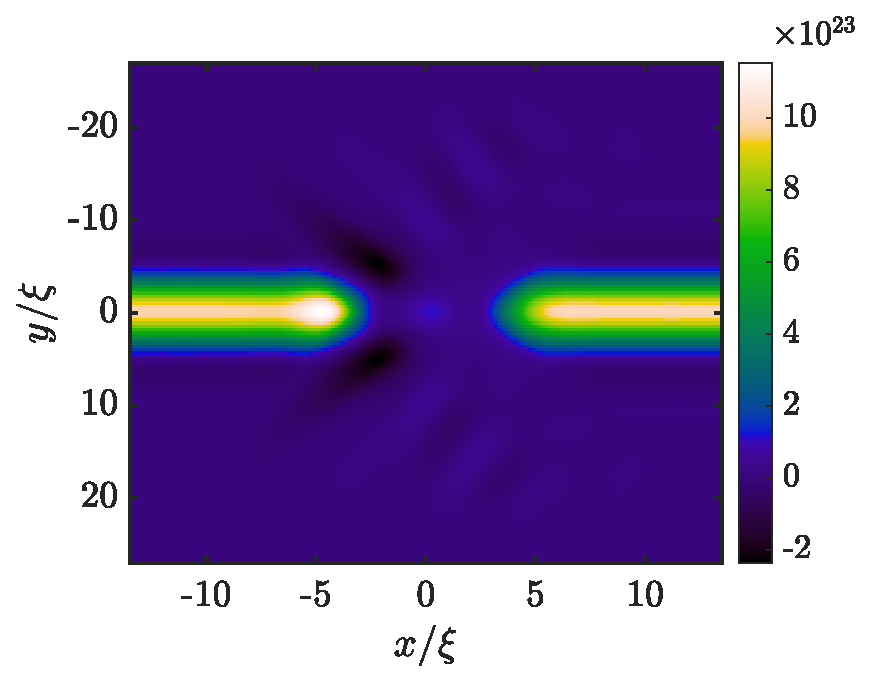
\includegraphics[width=\textwidth]{plots/section2/real_0.14V_Kx30_Nx4_Ky150_flat.eps}
        \caption[]%
        {{\small Realteil bei $U_2=\SI{0.14}{\volt}$.}}
        % \label{fig:G_3}
    \end{subfigure}
    \quad
    \begin{subfigure}[b]{0.48\textwidth}
        \centering
        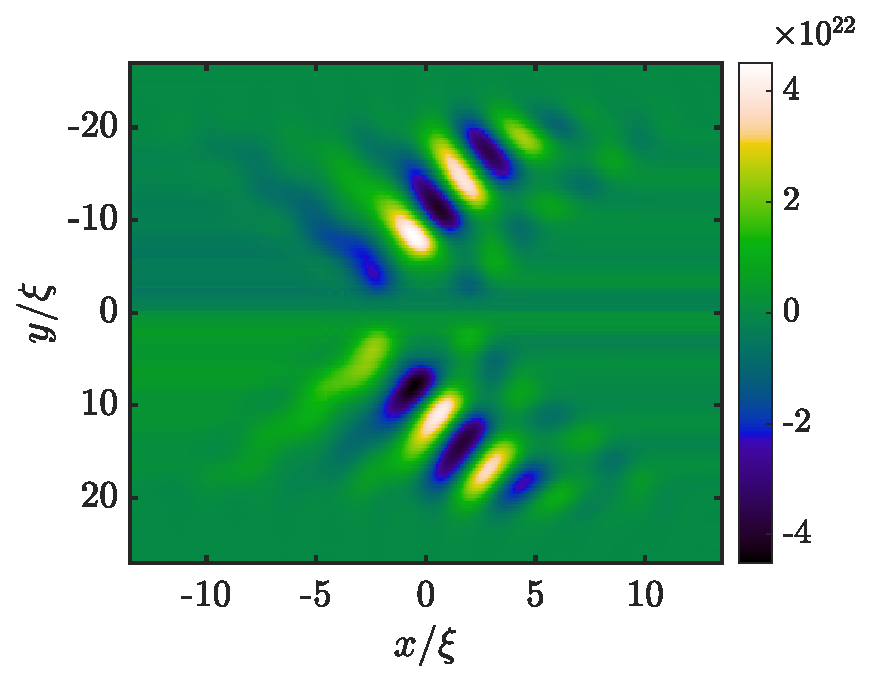
\includegraphics[width=\textwidth]{plots/section2/imag_0.14V_Kx30_Nx4_Ky150_flat.eps}
        \caption[]%
        {{\small Imaginärteil bei $U_2=\SI{0.14}{\volt}$.}}
        % \label{fig:G_4}
    \end{subfigure}
    \caption[]
    {Numerische Lösung für zwei verschiedene Spannungen, aufgeteilt in Imaginär- und Realteil. Parameter der Numerik: $K_x=30$, $N=4$, $K_y=150$. Physikalische Parameter: $L_x=\SI{66}{\nano\meter}$. Die Lösung wird an $400\times400$ äquidistant verteilten Punkten exakt ausgewertet.}
    \label{fig:solution}
\end{figure*}
Zum Vergleich ist in Abbildung \ref{fig:solution_gummel} das analoge Ergebnis einer selbstkonsistenten Rechnung (vgl. Kapitel \ref{sec:A_4}) zu sehen.
\begin{figure*}
    \centering
    \begin{subfigure}[b]{0.48\textwidth}
        \centering
        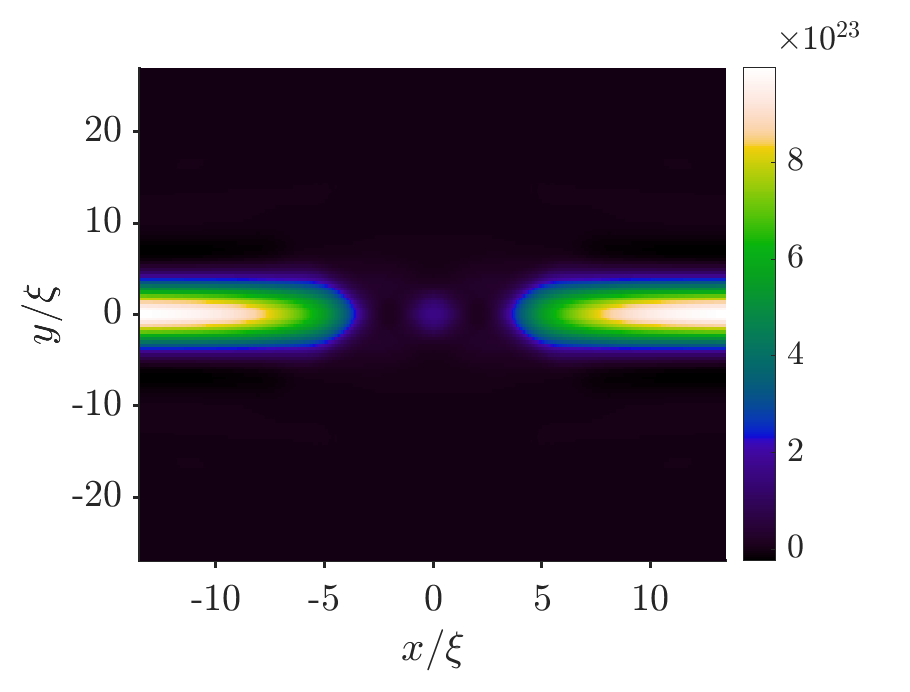
\includegraphics[width=\textwidth]{plots/section2/real_0.00V_Kx30_Nx4_Ky150_gummel_flat.eps}
        \caption[]%
        {{\small Realteil bei $U_1=\SI{0}{\volt}$.}}
        % \label{fig:G_1}
    \end{subfigure}
    \hfill
    \begin{subfigure}[b]{0.48\textwidth}
        \centering
        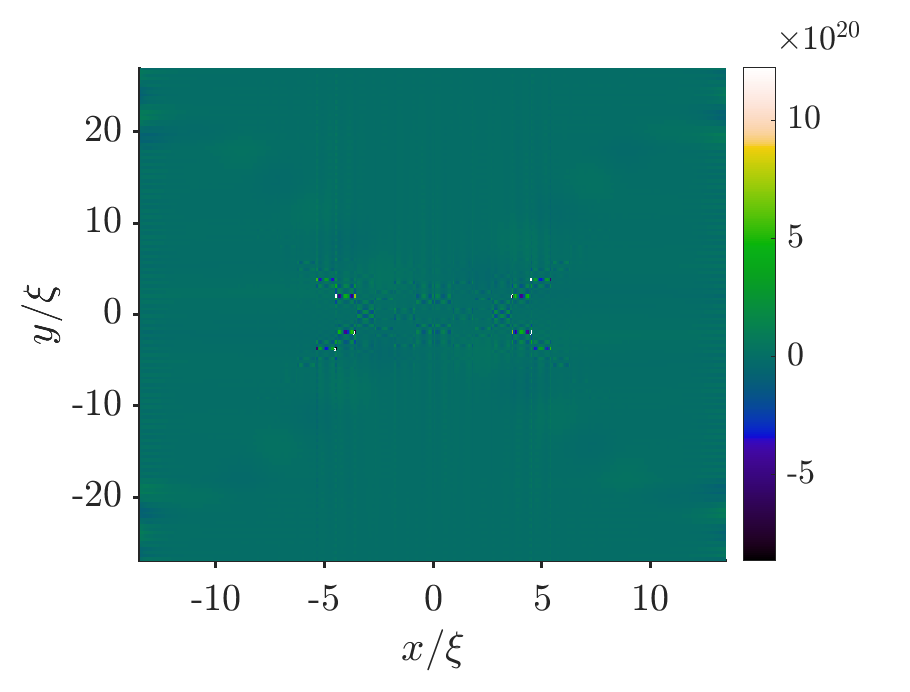
\includegraphics[width=\textwidth]{plots/section2/imag_0.00V_Kx30_Nx4_Ky150_gummel_flat.eps}
        \caption[]%
        {{\small Imaginärteil bei $U_1=\SI{0}{\volt}$.}}
        % \label{fig:G_2}
    \end{subfigure}
    \vskip\baselineskip
    \begin{subfigure}[b]{0.48\textwidth}
        \centering
        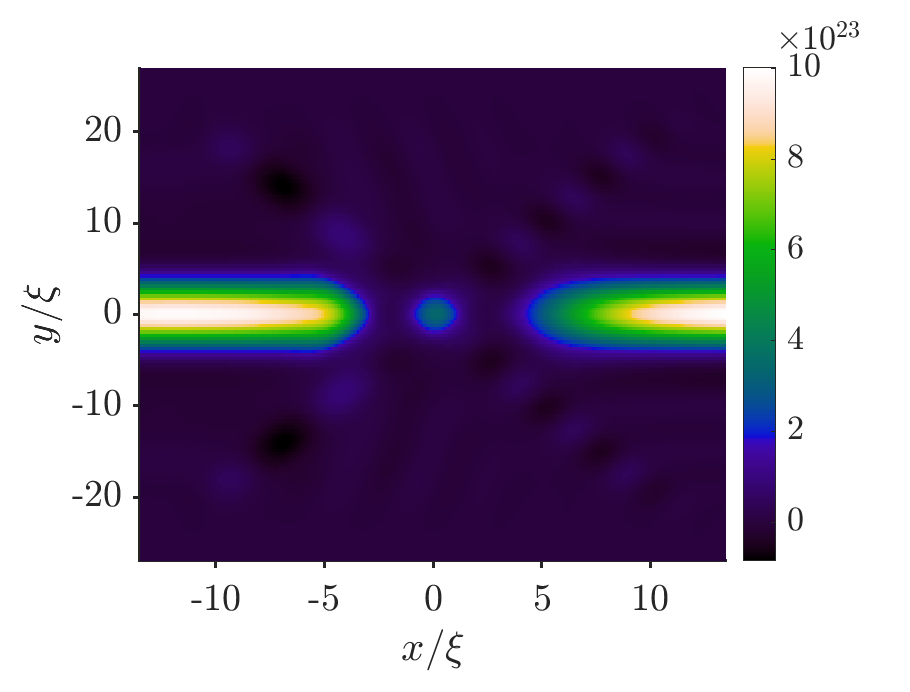
\includegraphics[width=\textwidth]{plots/section2/real_0.14V_Kx30_Nx4_Ky150_gummel_flat.eps}
        \caption[]%
        {{\small Realteil bei $U_2=\SI{0.14}{\volt}$.}}
        % \label{fig:G_3}
    \end{subfigure}
    \quad
    \begin{subfigure}[b]{0.48\textwidth}
        \centering
        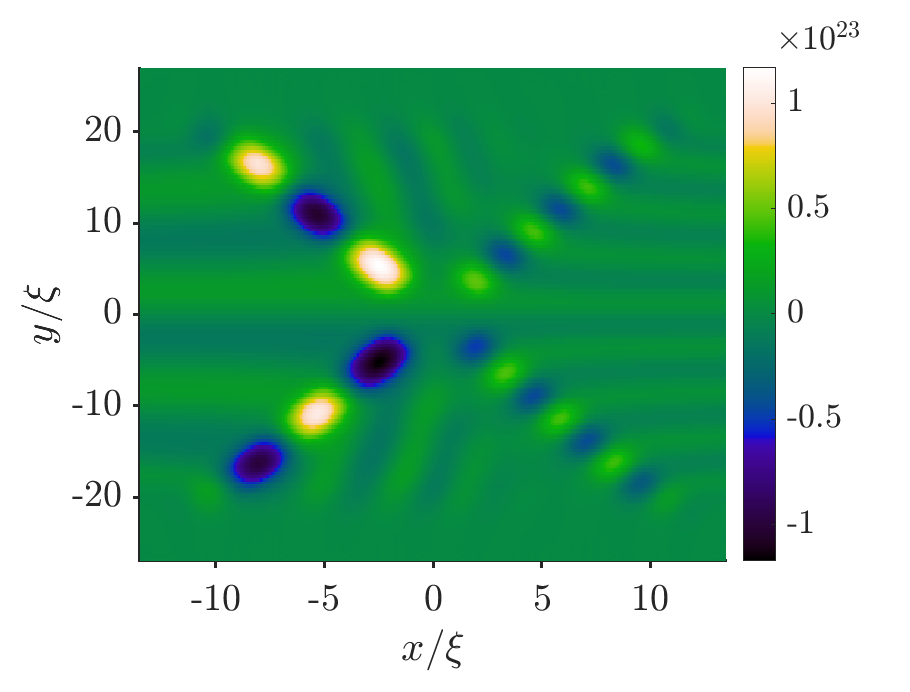
\includegraphics[width=\textwidth]{plots/section2/imag_0.14V_Kx30_Nx4_Ky150_gummel_flat.eps}
        \caption[]%
        {{\small Imaginärteil bei $U_2=\SI{0.14}{\volt}$.}}
        % \label{fig:G_4}
    \end{subfigure}
    \caption[]
    {Selbstkonsistente Rechnung mit ansonsten gleichen Parametern wie in Abbildung \ref{fig:solution}.}
    \label{fig:solution_gummel}
\end{figure*}
Die gezeigten Ergebnisse decken sich qualitativ mit den Ergebnissen anderer Verfahren wie einem \ac{fv}/\ac{fv}-Hybridverfahren in \cite{lukas1} oder einem Upwind-Differenzen-Schema für die Wignergleichung wie in \cite{frensley2}. Ein quantitativer Vergleich wird in Kapitel \ref{sec:rates} mit Hilfe der \ac{tf} aus Kapitel \ref{sec:TFmethod} vorgenommen. Ein Nachteil zeigt sich für den Imaginärteil im Gleichgewichtsfall bei $U_1=\SI{0}{\volt}$. Andere Verfahren (\ac{qtbm} und \ac{tf}) legen nahe, dass der Imaginärteil bis auf CPU-Genauigkeit verschwinden sollte, was hier nicht bestätigt werden kann.
Feinere Diskretisierungen verbessern zwar die Resultate diesbezüglich, jedoch konnte aufgrund begrenzter Rechenkapazität ein nomineller Unterschied zwischen Real- und Imaginärteil von ca. vier Größenordnungen nicht überschritten werden. Hier zeigt sich bereits, dass bezüglich des Imaginärteils eine Fehlerrate nach Gleichung \eqref{eq:optimaleKonvergenz} nicht erwartet werden kann.
\clearpage

\subsection{Strom-Spannungs-Kennlinien} 
Für einen qualitativen Vergleich werden im Folgenden Ergebnisse einer \ac{qtbm}-Rechnung (siehe \cite{qtbm}) mit einbezogen. Da die selbstkonsistente Rechnung für angelegte Spannungen keine gute Konvergenz zeigt, beschränken sich die Berechnungen auf Flachband-Modelle gemäß Abbildung \ref{fig:pot1}. Für den stationären Fall gilt wegen Gleichung \eqref{eq:kontigl} theoretisch $\partial_x j(x)=0$. Die numerischen Experimente zeigen jedoch, dass diese Forderung nicht perfekt eingehalten werden kann, siehe zum Beispiel Abbildung \ref{fig:kappa_var_4}. Eine mögliche Erklärung hierfür ist in der $y$-Diskretisierung zu finden, denn die Ableitung nach Gleichung \eqref{eq:ableitung_y} stellt lediglich eine grobe Näherung dar. Weitere Verfahren könnten eine $y$-Diskretisierung mit analytischer Ableitung\footnote{Eine analytische Ableitung kann mit stetigen Basisfunktionen gewährleistet werden.} implementieren, wie zum Beispiel ein \ac{fem}-Verfahren.
Da also ${j(x,t\rightarrow \infty)}$ nicht konstant ist entlang $x$, wird ein mittlerer Strom $j$ als Mittelwert gemäß
\begin{equation*}
  j \equiv \frac{1}{L_x} \int_{\Omega_x} \diff x j(x,t\rightarrow\infty)
\end{equation*}
definiert. Durch Iteration über verschiedene Spannungen ergibt sich die charakteristische Strom-Spannungs-Kennlinie einer \ac{rtd}, wie in Abbildung \ref{fig:iv1} zu sehen ist.
\begin{figure}
    \centering
    \begin{subfigure}[b]{0.47\textwidth}
        \centering
        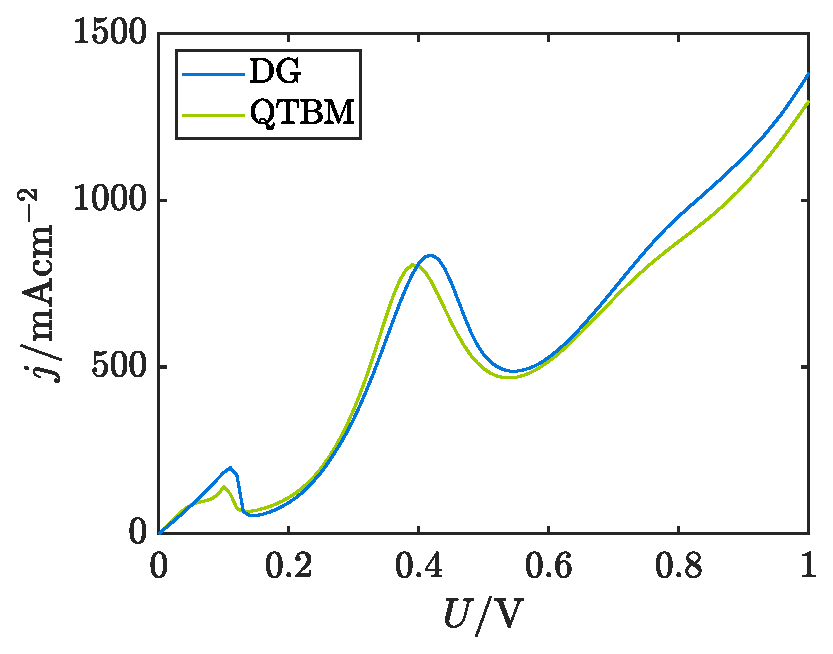
\includegraphics[width=\textwidth]{plots/IV/IV_qtbm_dg_grob.eps}
        \caption[]%
        {{}}
        \label{fig:iv1}
    \end{subfigure}
    \hfill
    \begin{subfigure}[b]{0.49\textwidth}
        \centering
        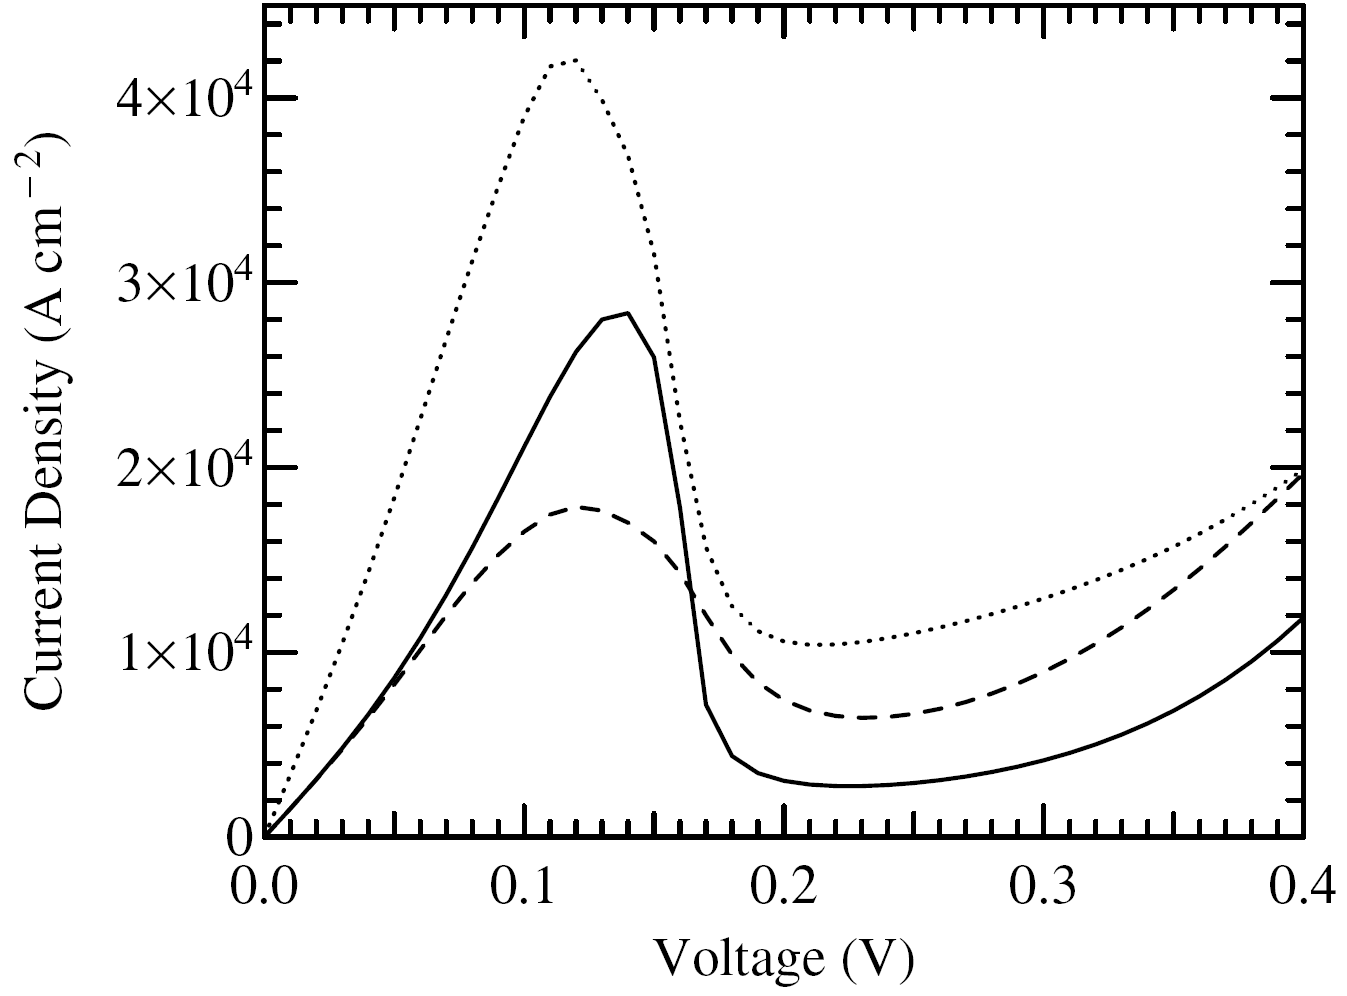
\includegraphics[width=\textwidth]{plots/IV/frensley.png}
        \caption[]%
        {{}}
        \label{fig:frensley_iv}
    \end{subfigure}
    \caption[]
    {Strom-Spannungs-Kennlinien im Vergleich. Parameter der Numerik: $K_x=30$, $N=7$, $K_y=280$. Zusätzlich gezeigt ist das Ergebnis einer \ac{qtbm}-Rechnung. Die Grafik rechts ist aus \cite{frensley3} entnommen. Die durchgezogene Linie ist das Resultat einer Tunneltheorie-Rechnung. Für die gestrichelte Linie wird eine lokale Variation der effektiven Masse berücksichtigt. Die punktierte Linie schließlich stellt das Ergebnis eines Modells mit nicht-lokaler effektiver Masse dar.}
    \label{fig:iv_vergleich1}
\end{figure}
Dabei ist für die \ac{qtbm}-Rechnung derselbe Parametersatz gewählt worden, während für die Grafik aus der Literatur \cite{frensley3} andere Parameter eingestellt sind. Es ist ersichtlich, dass die beiden Resonanzen bei ca. $\SI{0.11}{\volt}$ und $\SI{0.4}{\volt}$ reproduziert werden mit dem entwickelten \ac{dg}-Verfahren. Die Abbildung \ref{fig:frensley_iv} belegt dabei, dass sowohl Position als auch Höhe der Peaks abhängig sind von der zugrundeliegenden Theorie.

Auch innerhalb des \ac{dg}-Verfahrens gibt es einige variable Parameter, siehe Tabelle \ref{tab:parameter}. So lässt sich beispielsweise zwischen Methode G1 und G2 umschalten. Die entstehenden Unterschiede zeigt Abbildung \ref{fig:iv2} bei ansonsten gleichen Parametern.
\begin{figure}
  \centering
  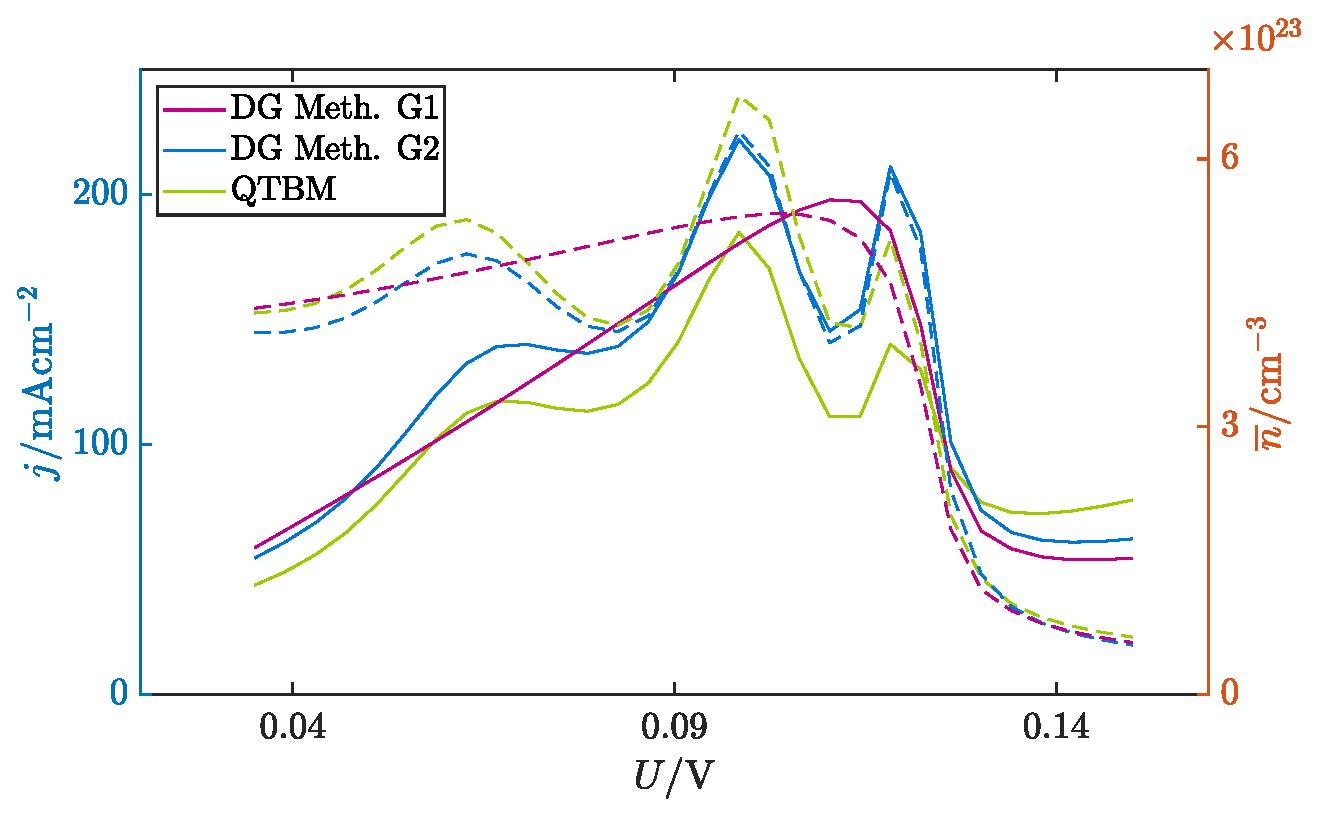
\includegraphics[width=0.8\textwidth]{plots/IV/IV_qtbm_dg_fein.eps}
  \caption{Auflösung des ersten Peaks bei ca. $\SI{0.1}{\volt}$ aus Abbildung \ref{fig:iv1}. Zum Vergleich ist zusätzlich das Ergebnis einer Rechnung mit Methode G2 gezeigt. Als gestrichelte Linie ist die gemittelte Teilchendichte $\overline{n}$ innerhalb des Quantentopfes dargestellt.}
  \label{fig:iv2}
\end{figure}
Anscheinend führt eine Approximation des Driftterms in höherer Ordnung zu Resultaten, die im Mittel etwas näher an der \ac{qtbm}-Lösung liegen. In beiden Fällen bilden sich jedoch statt einem Peak drei Peaks aus, die lediglich in der Höhe variieren. Möglicherweise ist auch dieses Problem auf die $y$-Diskretisierung zurück zu führen (siehe oben). Andererseits deutet der Verlauf der mittleren Dichte
\begin{equation*}
  \overline{n} \equiv \frac{1}{L_D} \int_{-L_D/2}^{+L_D/2} \diff x n(x,t\rightarrow\infty)
\end{equation*}
innerhalb des Quantentopfes (siehe Abbildung \ref{fig:iv2}) darauf hin, dass diese Begründung unzulänglich ist. Es ist nämlich zu erwarten, dass diese Größe dieselben resonanten Peaks zeigt, denn die Besetzung innerhalb des Quantentopfes ist ein Maß für die Zahl resonant besetzter Zustände \cite{frensley3}. Ein weiterer wichtiger Parameter könnte in diesem Zusammenhang $L_y$ sein, welcher ein Maß für die Ausdehnung ist, über die Quantenkorrelationen berücksichtigt werden.

Als nächstes werden daher die Parameter $L_x$ und $L_y$ variiert. Dabei zeigt sich sogar, dass die Ergebnisse mit Methode G1 teilweise zu negativen Stromflüssen führen. Dies ist ein klarer Indikator für die Problematik, die mit einer vergleichsweise groben Näherung des Driftterms einhergeht. Daher wird im Folgenden stets mit Methode G2 gerechnet (was einen rechnerischen Mehraufwand um einen Faktor neun in etwa mit sich bringt). Abbildung \ref{fig:iv3} zeigt das Resultat der Parametervariation im Bereich des ersten Peaks.
\begin{figure*}
    \centering
    \begin{subfigure}[b]{0.48\textwidth}
        \centering
        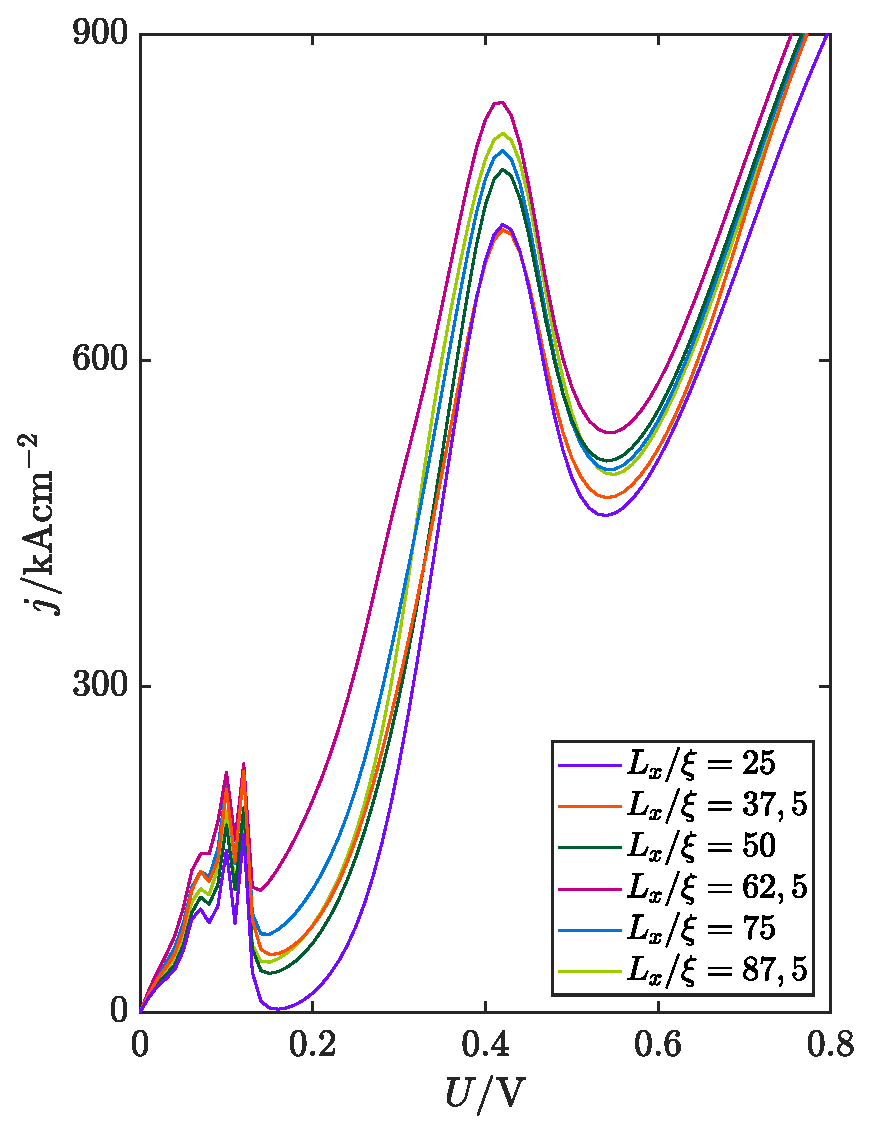
\includegraphics[width=\textwidth]{plots/IV/IV_Lx_variation.eps}
        \label{fig:iv3_1}
    \end{subfigure}
    \hfill
    \begin{subfigure}[b]{0.48\textwidth}
        \centering
        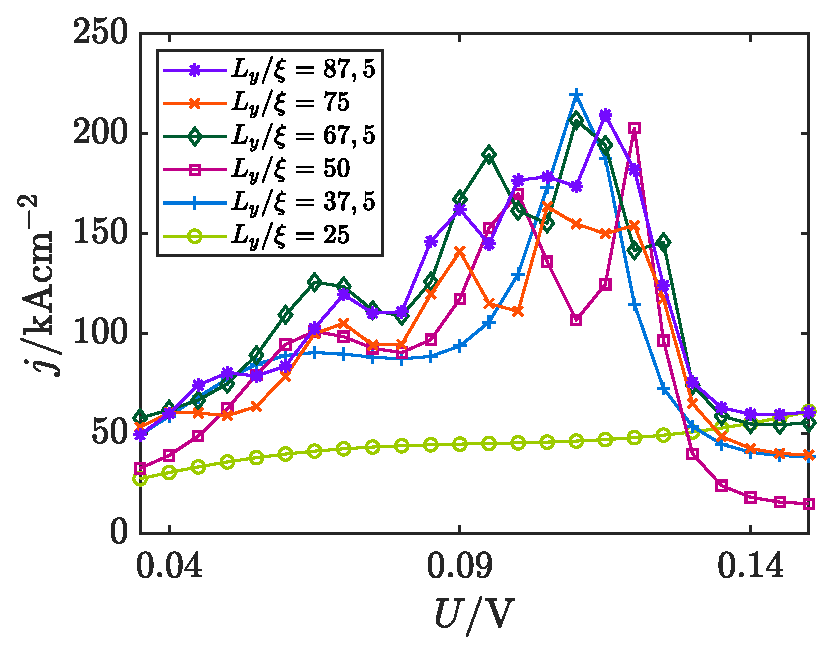
\includegraphics[width=\textwidth]{plots/IV/IV_Ly_variation.eps}
        \label{fig:iv3_2}
    \end{subfigure}
    \caption[]
    {Parametervariation bezüglich $L_x$ (links) und $L_y$ (rechts). Parameter der Numerik: $K_x=60$, $N=2$. Links ist  $K_y=180$ zudem konstant. Die Ausdehnung des \ac{cap} wird mit $\delta/\xi=8,3$ fixiert. Für die rechte Abbildung wird der Gitterabstand $h_y=L_y/K_y$ konstant gehalten, sodass keine Verzerrung bezüglich der Diskretisierung stattfindet.}
    \label{fig:iv3}
\end{figure*}
Offenbar haben beide Parameter einen Einfluss auf die Höhe des Peaks. Zusätzlich schwanken jedoch mit $L_y$ sowohl Position als auch Anzahl der Peaks. Genauer gesagt wird für $L_y/\xi=37,5$ lediglich ein Peak aufgelöst und mit steigendem $L_y$ kommen immer weitere Peaks hinzu, deren Amplituden zunehmend schwächer ausgeprägt sind. Dieses Verhalten deutet darauf hin, dass im Grenzfall großer Ausdehnung bei gleichzeitig feiner Diskretisierung tatsächlich nur noch ein Peak verbleibt.

Zusammenfassend bleibt festzuhalten, dass das Verfahren sehr sensibel auf den gewählten Parametersatz reagiert. Prinzipiell sind die Ergebnisse für die Strom-Spannungs-Kennlinie akzeptabel, jedoch stellt insbesondere die Auflösung des ersten Peaks ein  Problem dar. Die Herkunft der zusätzlichen Peaks kann nicht abschließend geklärt werden. Einen großen Einfluss wird hierbei auch das \ac{cap} haben, was möglicherweise in weiteren Arbeiten untersucht werden kann.

% Auch eine Variation bezüglich der numerischen Parameter erscheint daher sinnvoll und ist in Abbildung \ref{fig:iv4} gezeigt und quantitativ in Kapitel \ref{sec:rates} untersucht.
% \begin{figure}
%   \centering
%   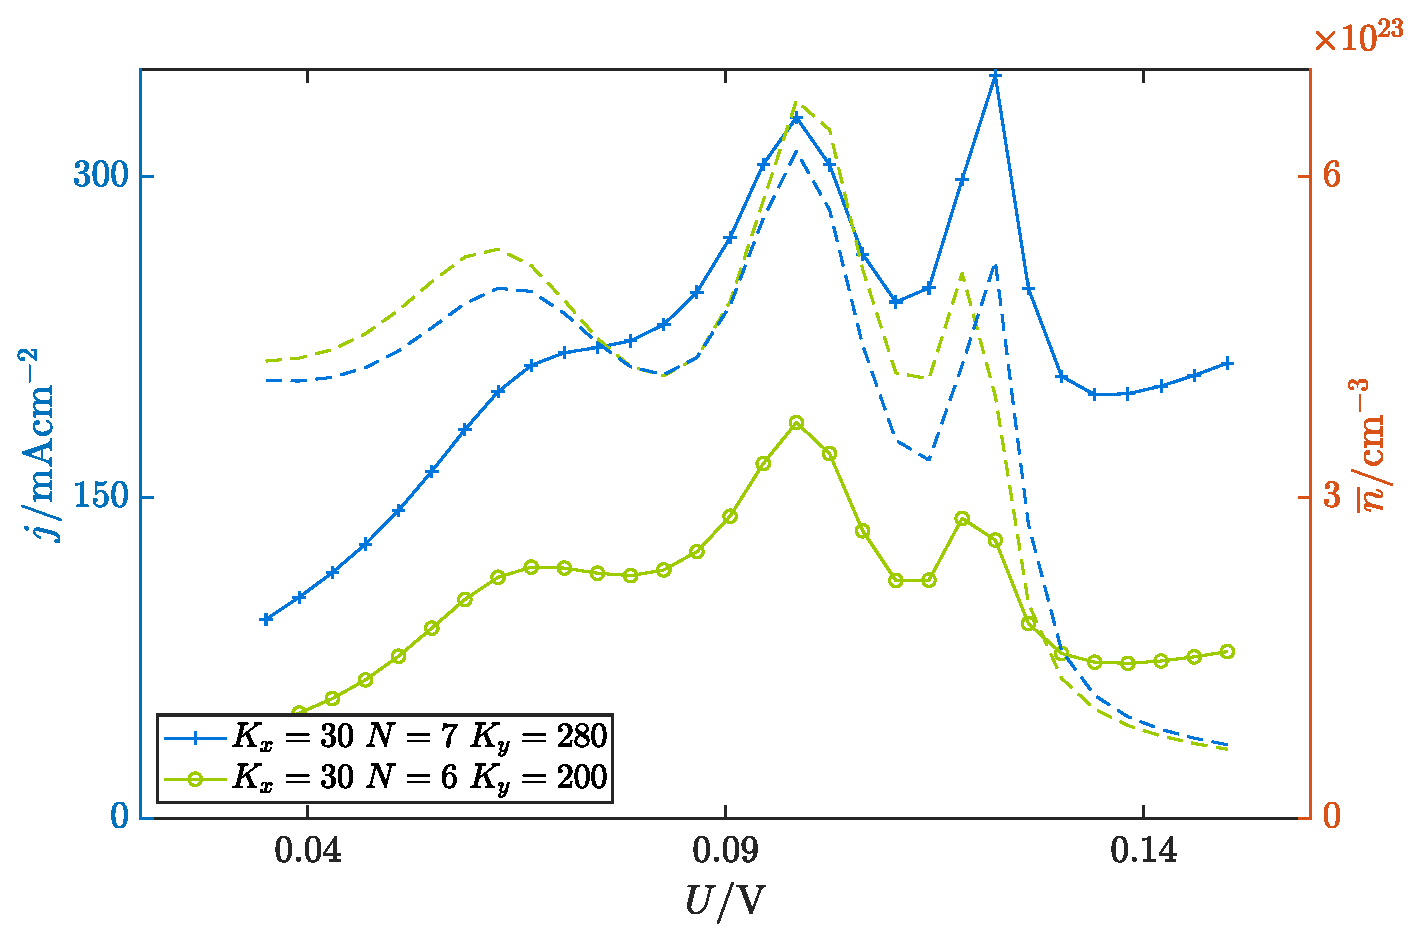
\includegraphics[width=0.8\textwidth]{plots/IV/IV_dg_vgl_diskretisierung_wide.eps}
%   \caption{Einfluss der Diskretisierung: Vergleich verschiedener Parameter der Numerik. Als gestrichelte Linie ist die gemittelte Teilchendichte $\overline{n}$ innerhalb des Quantentopfes dargestellt.}
%   \label{fig:iv4}
% \end{figure}
% Hier zeigt sich, dass die Höhe der Peaks schwankt, kaum hingegen deren Positionen.


\subsection{Einfluss des Strafparameters} \label{sec:kappa_var}
Neben den beiden für die Feinheit der Diskretisierung verantwortlichen Parametern $K_x$ und $N$ bietet das entwickelte \ac{dg}-Verfahren die Wahl des Strafparameters $\kappa$, siehe Gleichung \eqref{eq:numflux}. Aufgrund der Transport-Charakteristik der \ac{lvn} ist zu erwarten, dass ein Upwind-Fluss \index{Upwind-Fluss} die beste Approximation an den echten Fluss darstellt. Diese Erwartung wird anhand der Abbildung \ref{fig:kappa_var} bestätigt.
\begin{figure*}
    \centering
    \begin{subfigure}[b]{0.48\textwidth}
        \centering
        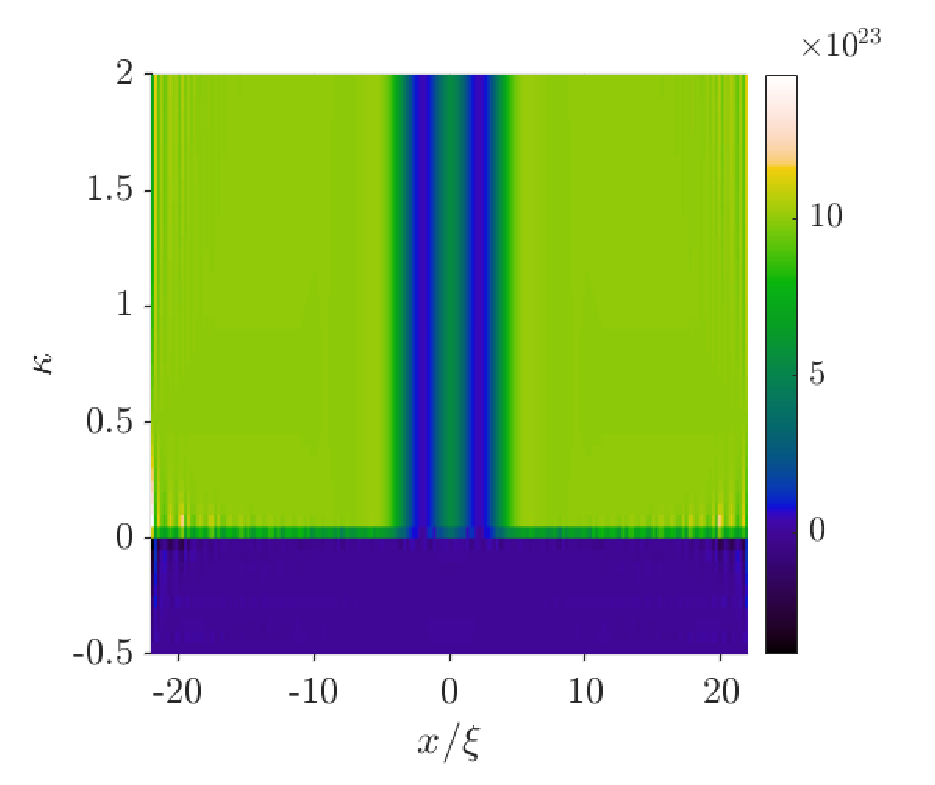
\includegraphics[width=\textwidth]{plots/kappa/kappa_variation_0V_n.eps}
        \caption[]%
        {{\small $n(x,\kappa)$ in m$^{-3}$ bei $U_1=\SI{0}{\volt}$.}}
        % \label{fig:G_1}
    \end{subfigure}
    \hfill
    \begin{subfigure}[b]{0.48\textwidth}
        \centering
        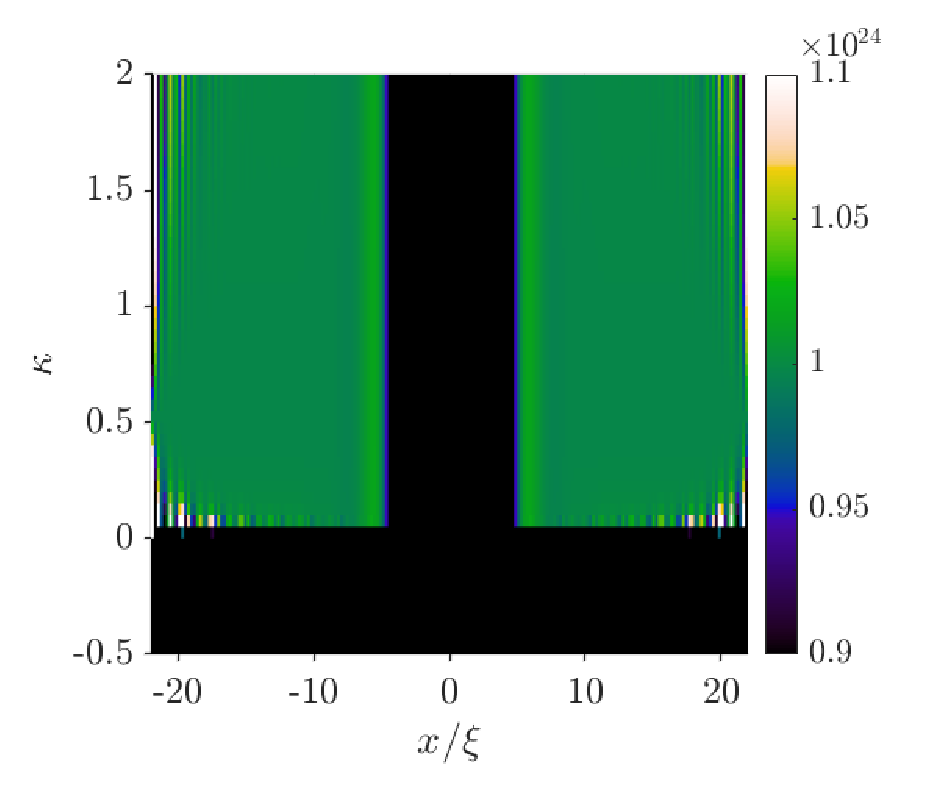
\includegraphics[width=\textwidth]{plots/kappa/kappa_variation_0V_n_zoomed.eps}
        \caption[]%
        {{\small Auflösung der Oszillationen.}}
        % \label{fig:G_2}
    \end{subfigure}
    \vskip\baselineskip
    \begin{subfigure}[b]{0.48\textwidth}
        \centering
        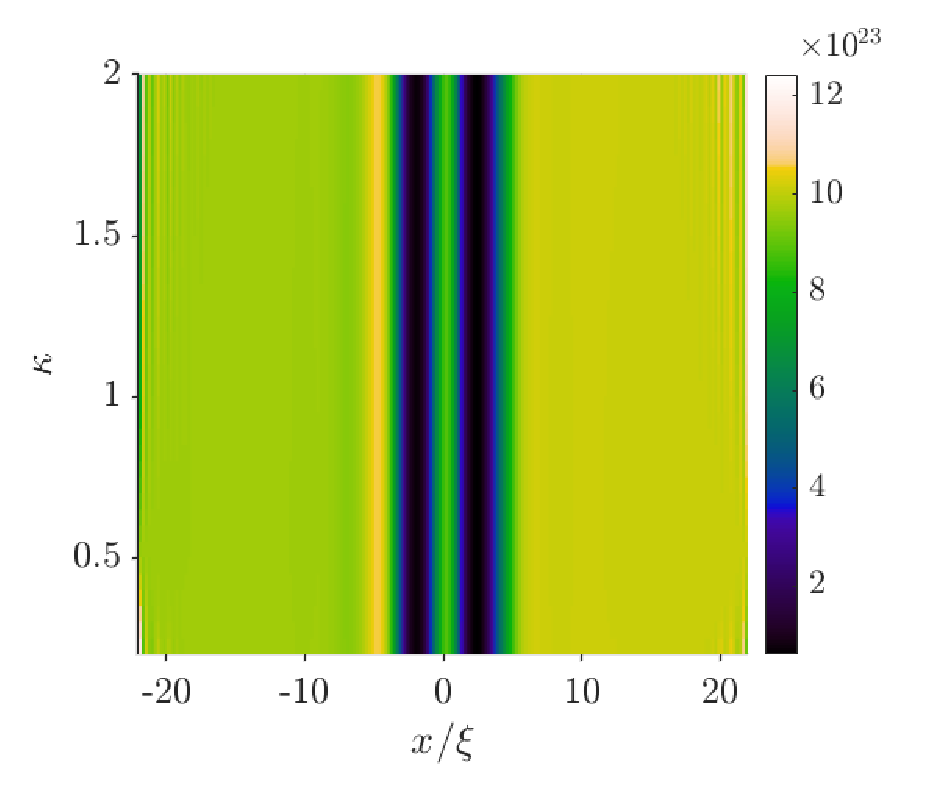
\includegraphics[width=\textwidth]{plots/kappa/kappa_variation_0.1V_n.eps}
        \caption[]%
        {{\small $n(x,\kappa)$ in m$^{-3}$ bei $U_2=\SI{0.1}{\volt}$ und akzeptablen Werten für $\kappa$.}}
        % \label{fig:G_3}
    \end{subfigure}
    \quad
    \begin{subfigure}[b]{0.48\textwidth}
        \centering
        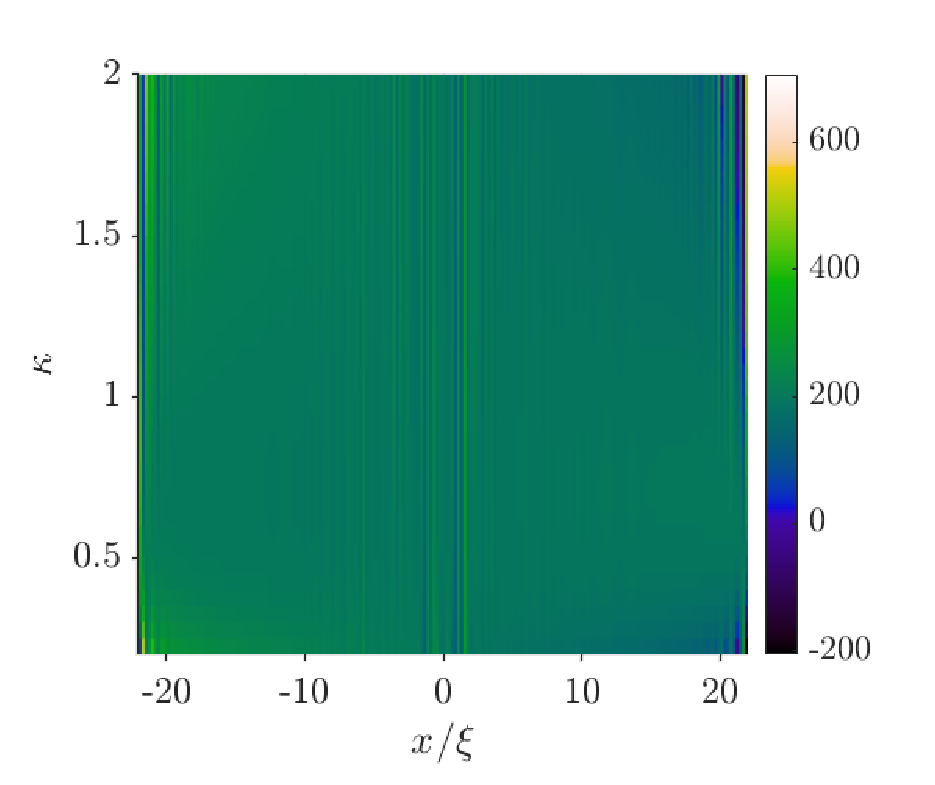
\includegraphics[width=\textwidth]{plots/kappa/kappa_variation_0.1V_j.eps}
        \caption[]%
        {{\small $j(x,\kappa)$ in kAcm$^{-2}$ bei $U_2=\SI{0.1}{\volt}$ und akzeptablen Werten für $\kappa$.}}
        \label{fig:kappa_var_4}
    \end{subfigure}
    \caption[]
    {Variation des Strafparameters $\kappa$.}
    \label{fig:kappa_var}
\end{figure*}
Es zeigt sich, dass es sowohl für $j(x)$, als auch für $n(x)$ im Bereich eines zentralen Flusses $\kappa=0$ zu starken Oszillationen kommt. Für negatives $\kappa$ bricht das Verfahren vollständig zusammen, wie dies auch durch die Existenz-Analyse aus Kapitel \ref{sec:existenz} vorausgesagt wird. Genauere Betrachtungen für $\kappa>0$ zeigen die beiden rechten Teile der Abbildung. Es ist klar zu erkennen, dass es insbesondere am Randbereich $x\approx \pm L_x/2$ zu Oszillationen kommt, wenn $\kappa\neq 0,5$.



\section{Konvergenzordnung der stationären Lösung}\label{sec:rates}
Für eine quantitative Analyse wird ein Vergleich des \ac{dg}-Verfahrens mit der \ac{tf} gezogen. Die Lösung der \ac{tf} wird als analytische Lösung gesetzt und der Fehler nach Gleichung \eqref{eq:error_ana} berechnet. Das Resultat ist in Abbildung \ref{fig:rates1} zu sehen.
\begin{figure*}
    \centering
    \begin{subfigure}[b]{0.48\textwidth}
        \centering
        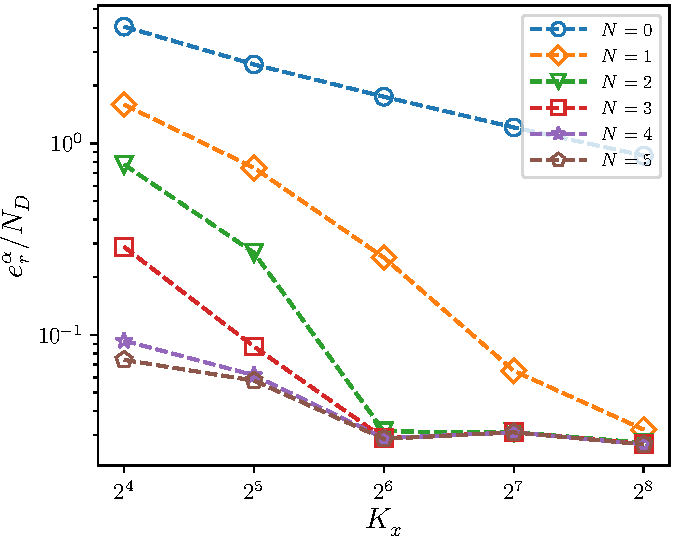
\includegraphics[width=\textwidth]{plots/test3/real_GL1.pdf}
        \label{fig:rates1_1}
    \end{subfigure}
    \hfill
    \begin{subfigure}[b]{0.48\textwidth}
        \centering
        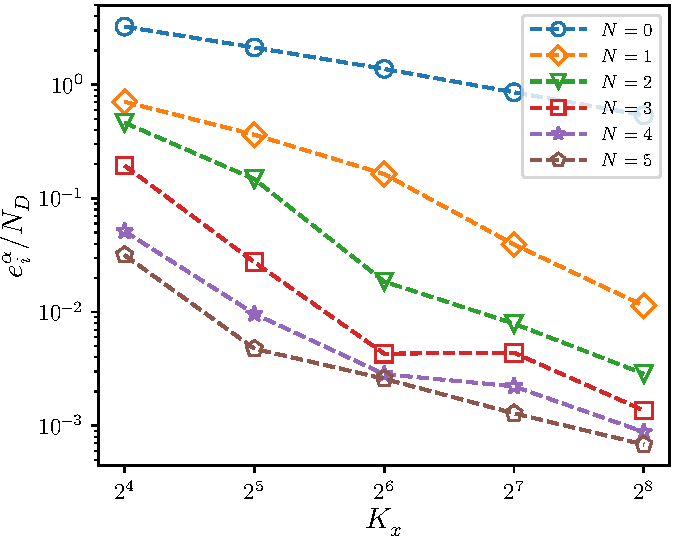
\includegraphics[width=\textwidth]{plots/test3/imag_GL1.pdf}
        \label{fig:rates1_2}
    \end{subfigure}
    \caption[]
    {Analytischer Fehler $e_{\nicefrac{r}{i}}$ mit der Lösung aus der \ac{tf} als exakte Lösung.}
    \label{fig:rates1}
\end{figure*}
Es zeigt sich eine sehr schwache Konvergenz, wobei nicht sichergestellt ist, ob es überhaupt zu einer Konvergenz im wörtlichen Sinne kommt. Vielmehr scheint es bezüglich des Realteils eine Art konstante Differenz zu geben. Die zugehörigen Fehlerraten sind
\begin{equation*}
  \begin{aligned}
    r_r &= \{0.58\pm0.05,\; 1.54\pm0.35,\; 1.55\pm1.26,\; 1.07\pm0.83,\; 0.53\pm0.49,\; 0.42\pm0.46\} \\
    r_i &= \{0.64\pm0.03,\; 1.39\pm0.48,\; 1.96\pm0.75,\; 1.82\pm1.31,\; 1.51\pm0.86,\; 1.54\pm0.85\} \\
    r_{\mathcal{T},r} &= \{0.36\pm0.13,\; 1.14\pm0.75,\; 1.41\pm1.21,\; 1.66\pm0.49,\; 1.47\pm0.83,\; 1.45\pm0.8\}
  \end{aligned}
\end{equation*}
und damit weit entfernt von der optimalen Konvergenz \eqref{eq:optimaleKonvergenz}. Es ist noch anzumerken, dass die Raten für Methode G1 noch schlechter sind. Die Suche nach möglichen Erklärungen führt unter Anderem auf die Frage nach der Form des Potentials. Im Wigner-Formalismus muss das Potential gefaltet werden und es bereitet dort wegen des Gibbschen Phänomens Schwierigkeiten, dieses nicht-lokale Faltungsintegral für eine Rechteckfunktion auszwerten. Ein möglicher Ansatz zur Umgehung des Problems ist dann die Glättung des Potentials, wie beispielsweise in \cite{wiedenhaus} geschehen.

Dieser Idee wird nachgegangen, indem das Potential $V^s$ mit einer Gauß-Funktion gefaltet und damit geglättet wird (der entsprechende Parameter ist in Tabelle \ref{tab:parameter} mit doPotConv gekennzeichnet). Das Ergebnis für die iterativen Fehler\footnote{Die \ac{tf}-Methode geht von einem Flachbandpotential aus und ist daher nun nicht mehr verfügbar.} ist in Abbildung \ref{fig:rates2} gezeigt.
\begin{figure*}
    \centering
    \begin{subfigure}[b]{0.48\textwidth}
        \centering
        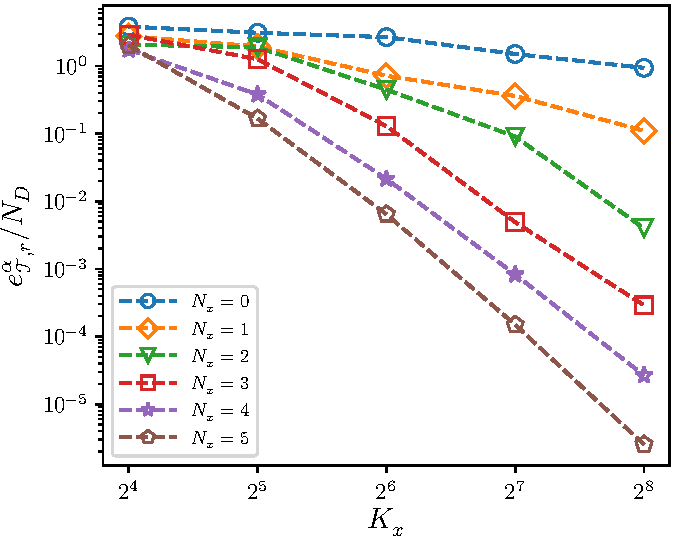
\includegraphics[width=\textwidth]{plots/test5/convGL1.pdf}
        \label{fig:rates2_1}
    \end{subfigure}
    \hfill
    \begin{subfigure}[b]{0.48\textwidth}
        \centering
        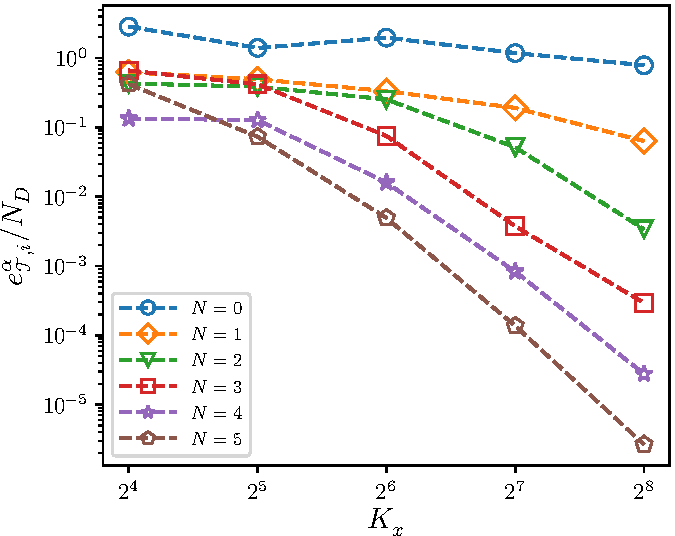
\includegraphics[width=\textwidth]{plots/test5/convGL1_i.pdf}
        \label{fig:rates2_2}
    \end{subfigure}
  \caption{Iterativer Fehler für die \ac{lvn} mit geglättetem Potential.}
  \label{fig:rates2}
\end{figure*}
Die zugehörigen Fehlerraten sind
\begin{align*}
  r_{\mathcal{T},r} &= \{0.45\pm0.27,\; 0.98\pm0.38,\; 1.5\pm0.98,\; 3.07\pm1.44,\; 3.68\pm1.07,\; 4.57\pm0.75\} \\
  r_{\mathcal{T},i} &= \{0.42\pm0.66,\; 0.57\pm0.19,\; 1.02\pm0.92,\; 2.49\pm1.5,\; 2.44\pm1.76,\; 3.86\pm1.08\} \; .
\end{align*}
Ab einer Systemgröße von etwa $K_x N \approx 160$ wird darüber hinaus nahezu optimale Konvergenz erreicht, wie die Abbildung bereits vermuten lässt.



\section{Transiente Lösung}\label{sec:transient}
In diesem Abschnitt wird die Antwort des Systems auf die zwei zeitlich variierenden Eingangsspannungen
\begin{align*}
  U_1(t) &= \begin{cases} U_A & t\leq 0 \\ (U_B - U_A)\frac{t}{t_\text{ramp}} & 0<t<t_{\text{ramp}} \\ U_B & t>t_{\text{ramp}} \end{cases} \\
  U_2(t) &= U_C \sin(2\pi f t)
\end{align*}
untersucht. Dabei werden die Konstanten zu
\begin{align*}
  U_A &= \SI{0.1}{\volt} & U_B &= \SI{0.2}{\volt} & U_C &= \SI{0.3}{\volt} \\
  t_{\text{ramp}}/\tau &= 6  & f \cdot \tau &= 0,013 & \text{(entspricht }&\SI{400}{\giga\hertz}\text{)}
\end{align*}
gewählt. Für den ersten Fall ergibt sich mit $t_{\text{ramp}}\rightarrow 0$ die Frage nach der \emph{Sprung-antwort}\index{Sprungantwort} des Systems. In allen transienten Berechnungen wird die stationäre Lösung zu der Spannung $U(t=0)$ als Anfangsbedingung gesetzt.

Die Ergebnisse für Strom und Spannung sind in Abbildung \ref{fig:transient} zusammengestellt.
\begin{figure*}
    \centering
    \begin{subfigure}[b]{0.48\textwidth}
        \centering
        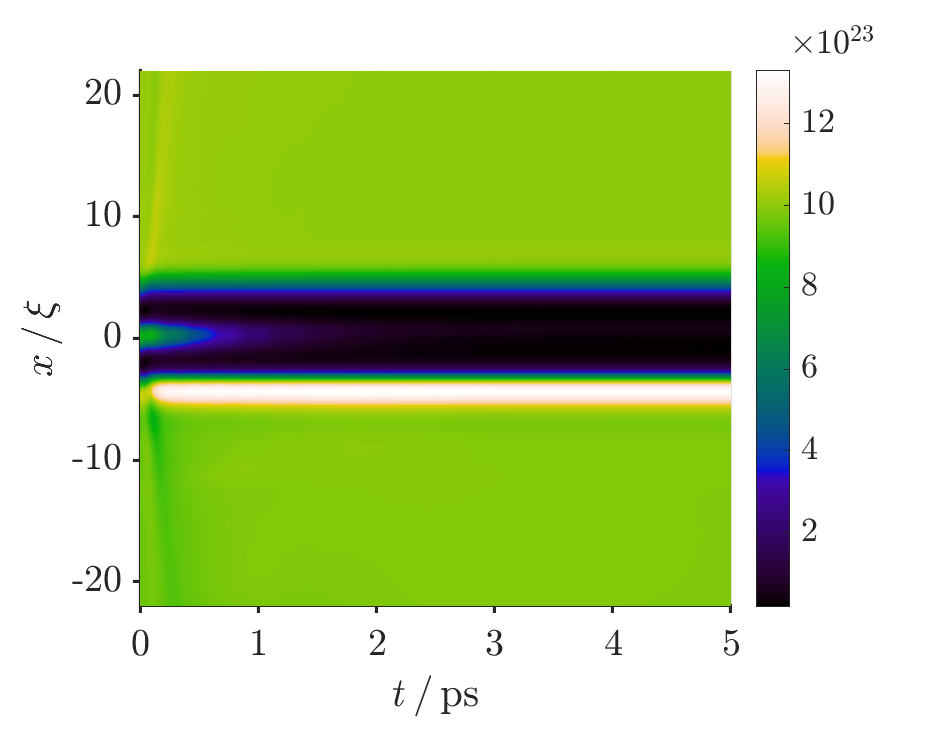
\includegraphics[width=\textwidth]{plots/transient/Dichte_sprung.eps}
        \caption[]%
        {{\small $n(x,t)$ in m$^{-3}$ bei $U_1(t)$.}}
        % \label{fig:G_1}
    \end{subfigure}
    \hfill
    \begin{subfigure}[b]{0.48\textwidth}
        \centering
        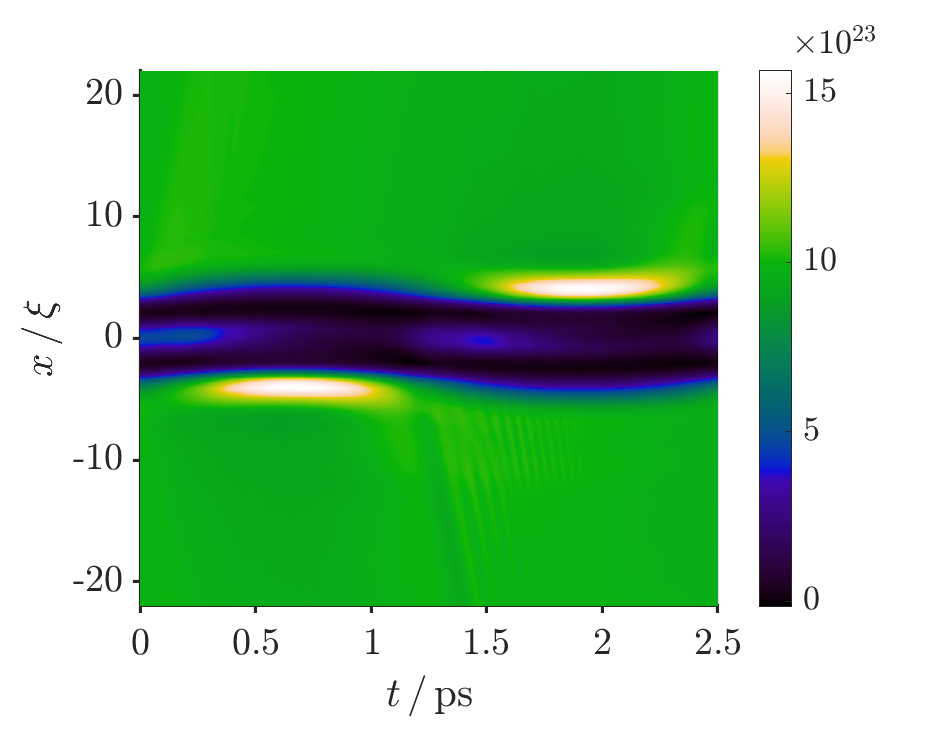
\includegraphics[width=\textwidth]{plots/transient/Dichte_sinus.eps}
        \caption[]%
        {{\small $n(x,t)$ in m$^{-3}$ bei $U_2(t)$.}}
        % \label{fig:G_2}
    \end{subfigure}
    \vskip\baselineskip
    \begin{subfigure}[b]{0.48\textwidth}
        \centering
        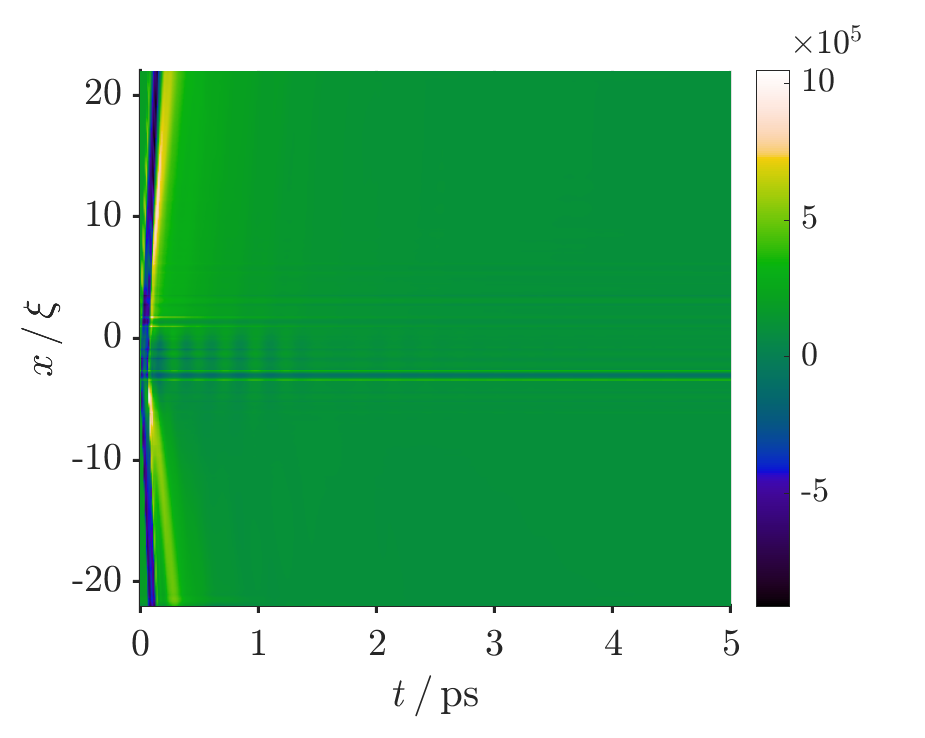
\includegraphics[width=\textwidth]{plots/transient/Strom_sprung.eps}
        \caption[]%
        {{\small $j(x,t)$ in m$^{-3}$ bei $U_1(t)$.}}
        % \label{fig:G_3}
    \end{subfigure}
    \quad
    \begin{subfigure}[b]{0.48\textwidth}
        \centering
        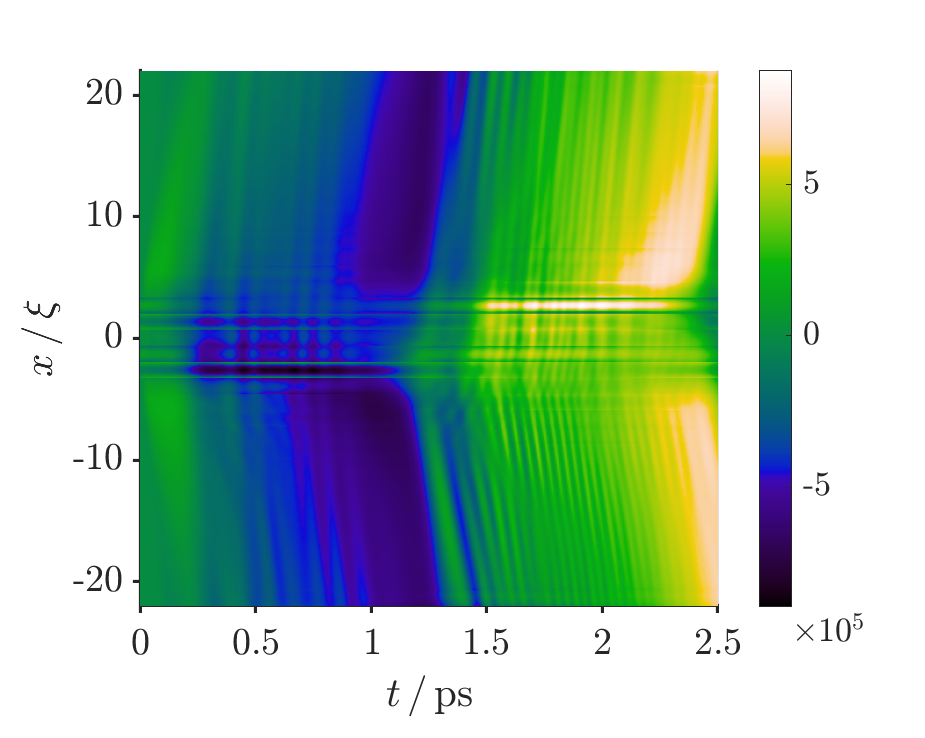
\includegraphics[width=\textwidth]{plots/transient/Strom_sinus.eps}
        \caption[]%
        {{\small $j(x,t)$ in m$^{-3}$ bei $U_2(t)$.}}
        % \label{fig:kappa_var_4}
    \end{subfigure}
    \vskip\baselineskip
    \begin{subfigure}[b]{0.48\textwidth}
        \centering
        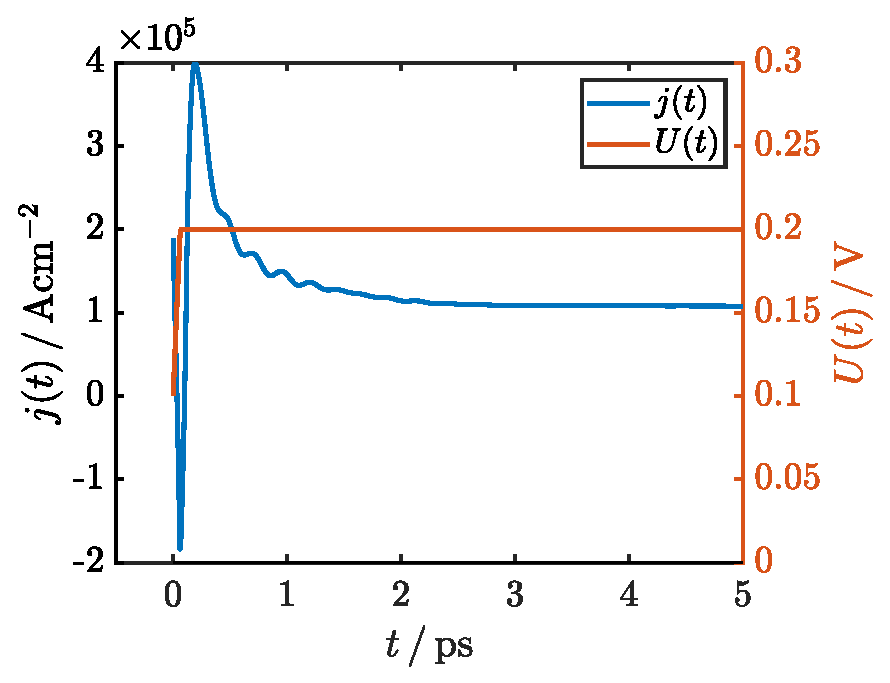
\includegraphics[width=\textwidth]{plots/transient/UI_sprung.eps}
        \caption[]%
        {{\small Strom- und Spannungsverlauf für $U_1(t)$.}}
        % \label{fig:G_3}
    \end{subfigure}
    \quad
    \begin{subfigure}[b]{0.48\textwidth}
        \centering
        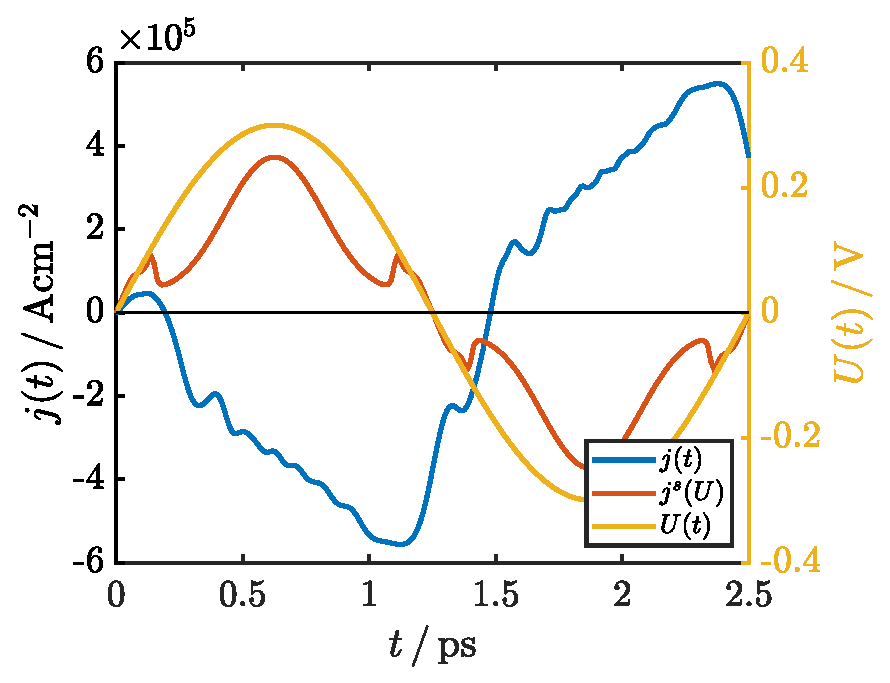
\includegraphics[width=\textwidth]{plots/transient/UI_sinus.eps}
        \caption[]%
        {{\small Strom- und Spannungsverlauf für $U_2(t)$.}}
        % \label{fig:transient_4}
    \end{subfigure}
    \caption[]
    {Zeitlicher Verlauf der Observablen. Links ist die Sprungantwort und rechts die Antwort auf eine Wechselspannung mit $f=\SI{400}{\giga\hertz}$ gezeigt. In den untersten Abbildungen ist zusätzlich zum gemessenen Strom der zu $U(t)$ korrespondierende stationäre Strom $j^s(U)$ eingezeichnet. Parameter der Numerik:  $K_x=33$, $N=2$, $K_y=100$.}
    \label{fig:transient}
\end{figure*}
Dabei ist das \ac{rk}2-Verfahren mit dem nach Formel \eqref{eq:delta_t} errechneten Zeitschritt ${\Delta t / \tau = 0,1036}$ (entspricht $\SI{0.3252}{\femto\second}$) zum Einsatz gekommen. Die Konstante $c$ in dieser Gleichung ist numerisch getestet worden. Es zeigt sich, dass es ab $c=1$ zu Instabilität kommt. Mit dahingegen restriktiv gewähltem $c=0,2$ hingegen treten keine Probleme auf.

Für das \ac{rk}2-Schema ist zu Testzwecken (wie in Kapitel \ref{sec:timestepping} erwähnt) ein gewisser Mehraufwand hinsichtlich \emph{Limiter} und \emph{strong stability preserving} implementiert worden. Die Verwendung eines \ac{rk}4-Schemas liefert keine Abweichungen gegenüber dem \ac{rk}2-Schema. Es kommt daher erwartungsgemäß zu keinen Problemen bezüglich Überschwingern in Folge nicht-stetiger Eingangsdaten.

Die Abbildung \ref{fig:transient} zeigt, dass das System bei einem Sprung der Spannung von $\SI{0.1}{\volt}$ auf $\SI{0.2}{\volt}$ nach einigen Überschwingern nach etwa $\SI{2}{\pico\second}$ auf den neuen stationären Zustand eingeschwungen ist. Es ist daher zu erwarten, dass die eingestellte Frequenz von $\SI{400}{\giga\hertz}$ zu hoch ist, als dass das System mit dem stationären Stromfluss $j^s(U)$ aus Abbildung \ref{fig:iv1} folgen könnte. Diese Erwartung bestätigt sich im rechten Teil der Abbildung. Es ist zu beobachten, dass der Strom bei positiver Spannung sogar negativ wird. Der Strom scheint der Spannung phasenverschoben zu folgen.

Hierzu ist anzumerken, dass die numerischen Parameter mit einer Systemgröße $K_xN=66$, $K_y=100$ eine relativ grobe Diskretisierung darstellen. Im letzten Kapitel ist gezeigt worden, dass die Fehlerraten erst ab etwa $K_x N \approx 160$ gute Konvergenz zeigen. Die aus der Ortsdiskretisierung resultierenden Fehler werden durch die Zeitentwicklung weiter verstärkt, sodass es zwangsläufig zu einem Abweichen von stationären Lösungen kommen muss für nicht-konstante Spannungen. Der Grund für die grob gewählte Diskretisierung wiederum ist schlicht in dem Rechenaufwand zu finden. Für eine zeitabhängige Spannung muss in jedem Zeitschritt die hoch-besetzte Matrix $\mathcal{G}$ (vergleiche Abbildung \ref{fig:G_1}) neu berechnet werden. Auch ein Zwischenspeichern und späteres Abrufen für bereits berechnete Spannungswerte ist nicht hilfreich aufgrund der immensen Datengröße. Mit einigem Aufwand könnte an dieser Stelle weiter optimiert werden.
